% don't remove the folling lines, and edit the defintion of \main if needed
%\documentclass[../report.tex]{subfiles}
%\providecommand{\main}{..}
%\IfEq{\jobname}{\currfilebase}{\AtEndDocument{\biblio}}{}
% until here
%\documentclass[12pt,twoside,a4paper]{cernrep} 
%\usepackage{rep_common}

%\usepackage[detect-all]{siunitx} 
%\usepackage{enumitem}
%\setlist{noitemsep}
%\usepackage{authblk}
%\usepackage[bookmarks, colorlinks=true, pdftex, linkcolor=blue, citecolor=blue,https://indico.cern.ch/event/765096/contributions/3295602/ urlcolor=blue]{hyperref}
%\usepackage[utf8]{inputenc}
%\usepackage{color}
%\usepackage{lscape}
%\usepackage{eurosym}

%\pagestyle{plain}
% --
% -- The bibliography file paths for the main volume and all parts
% --
%\def\bibfiles{\main/bib/chapter,\main/section1/bib/section,\main/section2/bib/section}
% --
%\providecommand{\biblio}{\nocite{article-minimal}\bibliographystyle{report}\clearpage\bibliography{\bibfiles}}  % *Modification: added `\main/` to specify relative file location.

\begin{document}
%\newcommand{\main}{.}
%\def\biblio{}

%\title{
%  Physics Briefing Book Accelerators Chapter \\ 
%  {\small for the Update of the European Strategy for Particle Physics 2019}
%  }
%\author{\rm 
\vspace*{-10mm}
\centerline{Input for the Update of the European Strategy for Particle Physics 2020} \\
\vspace*{9mm}
%{\it The Open Symposium in Granada (13--16 May 2019) was organized around 8 themes that are reflected in the corresponding chapters of this document, compiled by the following authors} \\
\begin{center}
{\vspace*{-3mm}\bf Electroweak Physics:}\quad \rm Richard Keith Ellis$^1$, Beate Heinemann$^{2,3}$ {\it (Conveners)} \\
Jorge de Blas$^{4,5}$, Maria Cepeda$^6$, Christophe Grojean$^{2,7}$, Fabio Maltoni$^{8,9}$, Aleandro Nisati$^{10}$, Elisabeth Petit$^{11}$, Riccardo Rattazzi$^{12}$, Wouter Verkerke$^{13}$ {\it (Contributors)}\\
{\vspace*{3mm}\bf Strong Interactions:}\quad \rm Jorgen D'Hondt$^7$, Krzysztof Redlich$^8$ {\it (Conveners)}\\
Anton Andronic, Ferenc Sikl\'{e}r {\it (Scientific Secretaries)} \\
Nestor~Armesto$^5$, Dani\"el~Boer$^6$, David~d'Enterria$^7$, Tetyana Galatyuk,  Thomas~Gehrmann $^8$, Klaus~Kirch$^9$, Uta~Klein$^{10}$, Jean-Philippe~Lansberg$^{11}$, Gavin P. Salam$^{12}$, Gunar Schnell$^{13}$, Johanna Stachel$^{14}$,  Tanguy~Pierog$^{15}$, Hartmut Wittig$^{16}$,   Urs~Wiedemann$^{17}${\it (Contributors)} \\
{\vspace*{3mm}\bf Flavour Physics:}\quad 
Belen Gavela, Antonio Zoccoli {\it (Conveners)} \\
Sandra Malvezzi, Ana Teixeira, Jure Zupan {\it (Scientific Secretaries)} \\
{\vspace*{3mm}\bf Neutrino Physics \& Cosmic Messengers:}\quad
Stan Bentvelsen, Marco Zito {\it (Conveners)} \\
Albert De Roeck $^4$, Bonnie Fleming $^5$, Francis Halzen $^6$, Andreas Haungs $^7$, Marek Kowalski$^8$, Susanne Mertens$^9$, Mauro Mezzetto$^{10}$, Silvia Pascoli$^{11}$, Bangalore~Sathyaprakash $^{12}$, Nicola~Serra $^{13}$, Thomas Schwetz$^7$ {\it (Contributors)} \\
{\vspace*{3mm}\bf Beyond the Standard Model:}\quad
Gian F.~Giudice, Paris Sphicas {\it (Conveners)} \\
Juan Alcaraz Maestre, Caterina Doglioni, Gaia Lanfranchi, Monica D'Onofrio, Matthew~McCullough, Gilad Perez, Philipp Roloff, Veronica Sanz, Andreas Weiler, Andrea~Wulzer~{\it(Contributors)} \\
{\vspace*{3mm}\bf Dark Matter and Dark Sector:}\quad
Shoji Asai, Marcela Carena {\it (Conveners)} \\
Babette D\"{o}brich, Caterina Doglioni, Joerg Jaeckel, Gordan Krnjaic, Jocelyn Monroe, Konstantinos Petridis, Christoph Weniger {\it (Scientific Secretaries)} \\
{\vspace*{3mm}\bf Accelerator Science and Technology:}\quad
Caterina Biscari, Leonid Rivkin {\it (Conveners)} \\
Philip Burrows, Frank Zimmermann {\it (Scientific Secretaries)}  \\
Michael Benedikt$^4$, Edda Gschwendtner$^4$, Erk Jensen$^{4}$, Mike Lamont$^{4}$,  Wim~Leemans$^7$,  Lucio~Rossi$^4$, Daniel Schulte$^4$, Mike Seidel$^2$, Vladimir Shiltsev$^6$, 
Steinar~Stapnes$^4$,  Akira~Yamamoto$^{4,5}$ {\it (Contributors)} \\
{\vspace*{3mm}\bf Instrumentation and Computing:}\quad
Xinchou Lou, Brigitte Vachon {\it (Conveners)} \\
Roger Jones, Emilia Leogrande {\it (Scientific Secretaries)} \\
Ian Bird$^4$, Amber Boehnlein$^5$, Simone Campana$^4$, Ariella Cattai$^4$, Didier~Contardo$^6$, Cinzia~Da~Via$^7$, Francesco Forti$^8$,  Maria Girone$^4$, Matthias~Kasemann$^9$, Weidon Li$^1$, Lucie~Linssen$^4$, Felix Sefkow$^9$, Graeme Stewart$^4$ {\it (Contributors)} \\
\vspace*{5mm}
{\bf Editors:\quad}Halina Abramowicz, Roger Forty, and the Conveners
\end{center}}

\institute{\footnotesize\vspace*{6mm}
$^1$ IPPP, University of Durham, Durham DH13LE, UK \\
$^2$ Deutsches Elektronen-Synchrotron (DESY), Hamburg, 22607, Germany \\
$^3$ Albert-Ludwigs-Universit\:{a}t Freiburg, Freiburg, 79104, Germany \\
$^4$ Centro de Investigaciones Energ\'{e}ticas, Medioambientales y Tecnol\'{o}gicas (CIEMAT), Avda.\ Complutense 40, 28040, Madrid, Spain \\
$^5$ Centre for Cosmology, Particle Physics and Phenomenology, Universit\'{e} catholique de Louvain, Louvain-la-Neuve, 1348, Belgium \\
$^6$ Dipartimento di Fisica e Astronomia, Universit\`{a}a di Bologna and INFN, Sezione di Bologna, via Irnerio 46, 40126 Bologna, Italy \\
{\it etc.\ for the other affiliations (to be completed for the next draft)}}


%\maketitle

%\begin{abstract}
%We summarize the accelerator physics and technology submitted to the 2019 Update of the European %Strategy for Particle Physics and presented at the Open Symposium in Granada. 
%\end{abstract}

% -- Set the level of the TOC: 2 means including subsection, 1 means
% including section 
%\setcounter{tocdepth}{2}
%\tableofcontents
%\newpage

% -- List of sections
% \subfile{\main/section1/section}
% \newpage
%\subfile{\main/section2/section}
%\newpage

\chapter{Accelerator Science and Technology}
% \section{Physics Briefing Book Accelerators Chapter for the Update of the European Strategy for Particle Physics 2019 
% }
\label{chap:acc}


%\section{Accelerator technology, role of other regions, strategies for after LHC, or after Higgs factory}

This chapter presents a summary of accelerator science and technology related submissions. Both state-of-the-art and challenges for the main technologies are highlighted. A summary of the expected performance of the future colliders considered in this document is given in Table~\ref{table:future-colliders}.

{\bf (better place for it, and for the time line for these projects given below in Figure 3, would be in the Executive Summary at the beginning of this document) -- Beate is checking the 350 GeV ILC option, whether it is included in the ILC CDR.}

The parameters and comparisons of the projects are based on the inputs submitted to the European Strategy Update, unless stated otherwise. Common assumptions have been made \cite{Bordry:2018gri} for the annual operating schedule of all colliders except ILC, CEPC and SPPC.

%\begin{landscape}
\begin{table}
\caption{Summary of the future colliders considered in this report. The number of detectors given is the number of detectors running concurrently, and only counting those relevant to the entire Higgs physics programme. The instantaneous and integrated luminosities provided are that used in the individual reports, and for $e^+e^-$ colliders the integrated luminosity corresponds to the sum of those recorded by the detectors. For HL-LHC this is also the case while for HE-LHC and FCC$_{hh}$ it corresponds to 75\% of that. The values for $\sqrt{s}$ are approximate, e.g.\ when a scan is proposed as part of the programme  this is included in the closest value (most relevant for the $Z$, $W$ and $t$ programme). For the polarisation, the values given correspond to the electron and positron beam, respectively. For HL-LHC, HE-LHC, FCC, CLIC and LHeC the instantaneous and integrated luminosity values are taken from Ref.~\cite{Bordry:2018gri}. For these colliders the number of seconds per year is $1.2\times 10^{7}$ based on CERN experience~\cite{Bordry:2018gri}. CEPC (ILC) assumes $1.3\times 10^{7}$ ($1.6\times 10^{7}$) seconds for the annual integrated luminosity calculation. When two values for the instantaneous luminosity are given these are before and after a luminosity upgrade planned.
The last column gives the abbreviation used in this report in the following sections. When the entire programme is discussed, the highest energy value label is used, e.g. ILC$_{500}$ or CLIC$_{3000}$. It is always inclusive, i.e.\ includes the results of the lower-energy versions of that collider. Also given are the shutdowns (SDs) needed between energy stages of the machine. SDs planned during a run at a given energy are included in the respective energy line.
\protect\\
{\bf Open questions:  
1) We need to check with the Higgs WG the ILC scenarios used: 350 GeV does not figure explicitly in the ILC submission document and inconsistent with our text (old line numbers) ---
Also Table 2: 250, 500, 1000. 
\label{table:future-colliders}}}
\begin{center}
\begin{tabular}{|l|ccccc|cc|l|} %\hline\hline
\hline\hline
Collider & Type & $\sqrt{s}$ & $\cal{P}$ [\%] & $N_{\rm Det}$& $\cal{L}_{\rm inst}$ & $\cal{L}$ & Time  & Ref.\\
& &  & [$e^-$/$e^+$] & & \small [$10^{34}$cm$^{-2}$s$^{-1}]$ & [ab$^{-1}$] & [years] &\\\hline
\rule{0pt}{1.0em}%
HL-LHC & $pp$ & 14\,TeV & - & 2 & 5 & 6.0 & 12 & \cite{Cepeda:2019klc} \\\hline
HE-LHC & $pp$ & 27\,TeV & - & 2 & 16 & 15.0 & 20 & \cite{Cepeda:2019klc}  \\\hline
FCC-hh & $pp$ & 100\,TeV & - & 2 & 30 & 30.0 & 25 & \cite{Mangano:FCC2018}  \\\hline
FCC-ee & $ee$ & $M_Z$ & 0/0 & 2 & 100/200 & 150 & 4 & \cite{Mangano:FCC2018}   \\
  & & $2M_W$ & 0/0 & 2 & 25 & 10 & 1-2 & \\
  & & $240$\,GeV & 0/0 & 2 & 7 & 5 & 3 & \\
  & & $2m_{top}$ & 0/0 & 2 & 0.8/1.4 & 1.5 & 5 & \\
    &  \multicolumn{4}{c}{(1y SD before $2m_{top}$ run)} &  & (+1) & & \\\hline
  ILC & $ee$ & $250$~GeV & $\pm 80$/$\pm 30$ & 1 & 1.35/2.7 & 2.0 & 11.5 & \cite{Fujii:2017vwa} \\
  & & $350$~GeV & $\pm 80$/$\pm 30$ & 1 & 1.6 & 0.2 & 1 & \cite{Bambade:2019fyw} \\
  & & $500$~GeV & $\pm 80$/$\pm 30$ & 1 & 1.8/3.6 & 4.0 & 8.5 & \\
  &  \multicolumn{4}{c}{(1y SD after 250 GeV run)} & & (+1) & & \\\hline
   CEPC & $ee$ & $M_Z$ & 0/0 & 2 & 17/32 & 16 & 2 & \cite{CEPCStudyGroup:2018ghi} \\
  & & $2M_W$ & 0/0 & 2 & 10 & 2.6 & 1 & \\
  & & $240$~GeV & 0/0 & 2 & 3 & 5.6 & 7 &  \\\hline
    CLIC & $ee$ & $380$~GeV & $\pm 80$/$0$ & 1 & 1.5 & 1.0 & 8 & \cite{Roloff:2018dqu}  \\
  & & $1.5$~TeV & $\pm 80$/$0$ & 1 & 3.7 & 2.5 & 7 & \\
  & & $3.0$~TeV & $\pm 80$/$0$ & 1 & 6.0 & 5.0 & 8 & \\
  &  \multicolumn{4}{c}{(2y SDs between energy stages)} & & (+4) & & \\\hline
   LHeC & $ep$ & 1.3\,TeV & - & 1 & 0.8 & 1.0 & 15  & \cite{Bordry:2018gri} \\\hline
   HE-LHeC & $ep$ & 1.8 \,TeV & - & 1 & 1.5 & 2.0 & 20 &  \cite{Mangano:FCC2018} \\\hline
   FCC-eh & $ep$ & 3.5\,TeV & - & 1 & 1.5 &  2.0 & 25 & \cite{Mangano:FCC2018} \\
\hline\hline
%\hline\hline
\end{tabular}
\end{center}
\end{table}
%\end{landscape}

\section{Present state of accelerator technology for HEP}

Both circular electron-positron and hadron colliders have operated or are operating at peak luminosities above 1--2$\times 10^{34}$~cm$^{-2}$s$^{-1}$. 
PEP-II, KEKB and LHC have all exceeded their design specifications in terms of peak performance. 

Today's colliders all operate with bunched beams.
Assuming the collision of beams with identical parameters,
and bunches colliding at an average frequency 
$f_{\rm coll}$, with $N_{b}$ particles per bunch, 
a basic expression for the luminosity is 
\begin{equation} \label{accel:eq:lum}
    L = f_{\rm coll} \frac{N_b^2 }{4\pi\sigma_x^{\ast} \sigma_y^{\ast}}
    =  f_{\rm coll} \frac{N_b^2}{4\pi \sqrt{\varepsilon_x\,\beta_x^*\,\varepsilon_y\,\beta_y^*}}
\end{equation}
where $\sigma_x^{\ast}$ and $\sigma_y^{\ast}$ designate the rms transverse beam 
sizes in the horizontal (bend) and vertical directions at the interaction point (IP), which can also be expressed in terms of the geometric emittances  and IP beta functions.     
In the above form, 
it is assumed that the bunches are identical in transverse profile,
that the profiles are Gaussian and independent of position along the bunch, and the particle
distributions are not altered during the 
bunch collision. 
Nonzero beam crossing angles $\theta_{c}$ in the horizontal plane and long bunches 
(rms bunch length $\sigma_{z}$) will reduce the luminosity from the above value, 
e.g.~by a factor $1/(1+\phi^{2})^{1/2}$, 
where the parameter
$ \phi \equiv \theta_{c} \sigma_{z}/(2 \sigma_{x}^{\ast})$ is known as the Piwinski angle,
but a large Piwinski angle angle may also allow for smaller beta function and higher bunch population. 
The disruption or pinch effects and the dynamic changes of beta functions and emittance (due to the collision) also modify the luminosity in linear and circular colliders, respectively. 
Various phenomena may limit the luminosity,
such as beamstrahlung, disruption, beam-beam tune shift, achievable beam power etc.
The above formulae can be recast in different forms according to the most relevant constraints.

For example, in the case of modern hadron colliders, like the HL-LHC the luminosity is often limited by the maximum acceptable detector pile up, and the luminosity then needs to be levelled at this value. 

In the case of circular $e^+e^-$ 
colliders the luminosity may be limited by the total synchrotron radiation power (determining the total beam current $I_{b}$) and the maximum beam-beam tune shift $\xi_y$, 
in which case the
luminosity formula can be rewritten as  
\begin{equation}
    L \propto \frac{\xi_y}{\beta_{y}^{\ast}} 
    \frac{P_{\rm SR}}{E_b^{3}} \; \, \, \ \text{(circular $e^+e^-$ colliders)}\, ,
\end{equation}
where $E_{b}$ denotes the beam energy. 
The maximum beam-beam tune shift $\xi_y$ increases
with beam energy, and also depends on the collision scheme.

In the case of linear e$^+$e$^-$ 
colliders it is convenient
to rewrite the luminosity expression as
\begin{equation}
L \propto H_{D} \frac{N_{b}}{\sigma_{x}^\ast}
\frac{1}{\sqrt{\beta_{y}^{\ast}\varepsilon_y}} I_{b}
\; \, \, \text{(linear $e^+e^-$ colliders)}\, ,
\end{equation}
where $H_{D}$ denotes the luminosity enhancement factor, which includes the geometry of the collision and the
beam-beam effects, and is of the order of one.
The factor $N_{b}/\sigma_{x}^{\ast}$ is proportional to the number of beamstrahlung photons emitted per beam particle; it determines the purity of the luminosity energy spectrum, which is constrained by
experimental requirements.
The last term $I_{b}$ 
is the average beam current $I_{b}=f_{\rm coll}  N_{b} e$ (with $e$ the electron charge),
and the collision rate $f_{\rm coll}$ equals the product of linac pulse 
rate and the number of bunches per pulse.

{\bf $pp$ colliders:} Between  2015 and 2018 (`Run 2') the LHC has accumulated 190 fb$^{-1}$ in proton-proton collisions. 
The goal for HL-LHC is to deliver about 0.25 ab$^{-1}$ per year with the aim of integrating a total luminosity in the range of 3 to 4.5 ab$^{-1}$ by the late 2030s. 
The beam current is above 0.55 A and the beta functions at the collision point are as low as 25 cm. Dipole {\bf magnets} of 11 T and quadrupole magnets with a peak pole field of 12 T, based on Nb3Sn superconductor, are under development for HL-LHC. As part of the US DOE magnet development program, a first prototype dipole magnet exceeded a field of 14 T at FNAL in late spring 2019. In parallel superconducting cables are being developed worldwide. In 2018-19, two independent US teams developed advanced Nb$_3$Sn cables with artificial pinning centers; these offer a 50\% higher critical current density than the HL-LHC cable and fulfil the target requirements for FCC. New suppliers in Japan, Korea and Russia have produced Nb$_3$Sn cables that meet the HL-LHC requirements, widening the base of potential manufacturers.


{\bf $e^+e^-$ colliders:} Between 1999 and 2008, the {\bf circular colliders (CC)} PEP-II and KEKB accumulated a total of almost 1.6 ab$^{-1}$, with beam currents at PEP-II as high as 2.1 A ($e^-$) and 3.2 A ($e^+$) and a vertical IP beta function at KEKB as low as 6 mm; their integrated luminosity  was greatly increased by the introduction of {\bf top-up} injection. SuperKEKB is presently being commissioned with a peak luminosity design goal of 
$8\times 10^{35}$~cm$^{-2}$s$^{-1}$. The {\bf crab-waist (CW)} collision scheme was demonstrated at DAFNE around 2008, where it substantially increased the peak luminosity, and is incorporated into all 
future circular $e^+e^-$ proposals. SLC at SLAC (1988--1998) is the first and only {\bf linear collider (LC)} implemented to date.   Since then significant R\&D has been performed on  high-gradient/high-frequency NC RF for CLIC and on SC RF for ILC (see below). Based on these technologies several high-energy linacs have been built to serve as X-ray FELs (SwissFEL, EU-XFEL, LCLS) and significant experience has been gained in beam tuning/focusing at test facilities (FACET, ATF/ATF2), demonstrating `nanobeam' feasibility for a future LC. ATF2 has achieved the scaled ILC vertical spot size of $\sim$~40 nm, 
albeit with a relaxed optics and at roughly 1/10 of the design bunch charge; the charge was reduced to mitigate wakefield effects. 

The world record for {\bf positron} production rates is still held by the SLC positron source. Figure~\ref{polsources} compares the demonstrated positron production at SLC, KEKB and SuperKEKB with the needs for future $e^+e^-$ colliders\cite{benedikt-granada,zimmermann-pol}. 
LCs require much higher positron production rates than SLC (CLIC about 20 times more, ILC baseline about 40 times, ILC upgrade about 160 times). The CLIC design incorporates a conventional positron source while the ILC baseline (for polarized positrons) passes the high-energy electron beam through a $\sim$100 m long undulator, generating photons that hit a rapidly rotating target to produce $e^+e^-$  pairs.


\begin{figure}[ht]
\centering
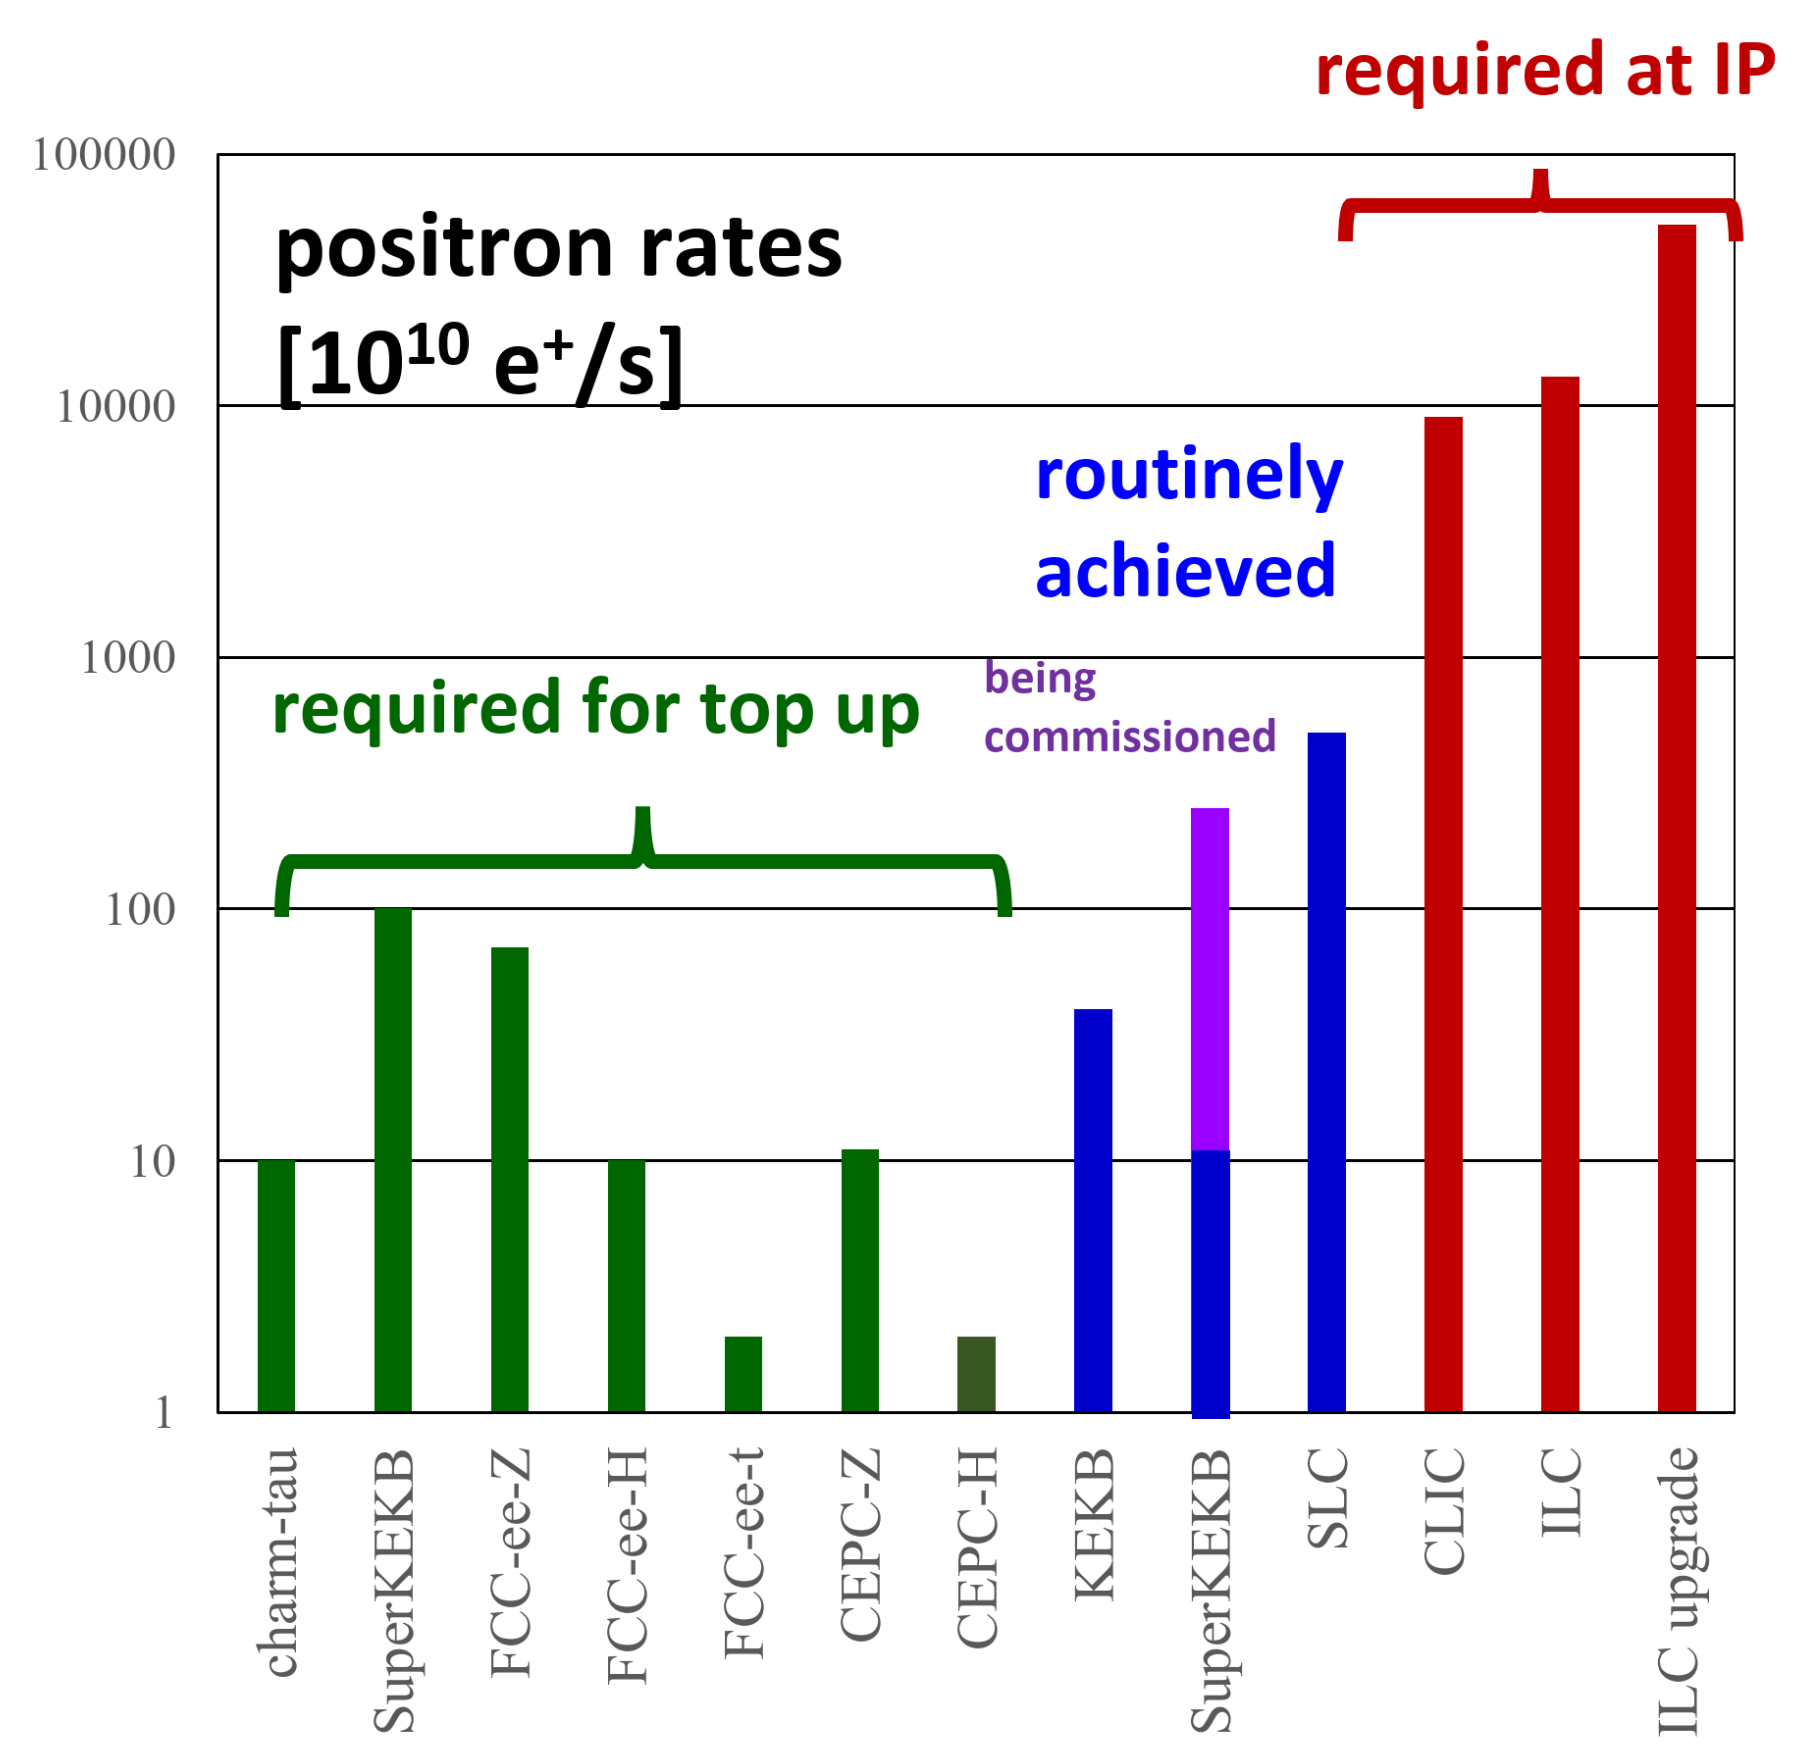
\includegraphics[width=0.60\textwidth]{\main/Accelerator/img/polsources.png}
\caption{Positron production rates achieved at the SLC, KEKB and SuperKEKB compared with those required for future $e^+e^-$ colliders. \label{polsources}.}
\end{figure}


\section{Technologies for electroweak sector} 

\paragraph*{$e^+e^-$ Higgs factories}

The Higgs production process in $e^+e^-$ colliders peaks at different energies according to the different channels, as shown in the chapter on Electroweak Physics (see Fig.~\ref{fig:xsec_vs_cme}). We call here Higgs factories the $e^+e^-$ colliders with c.o.m.~energies optimized for the maximum corresponding physics reach.

One can be confident that the energy goal can be reached for all the considered configurations. Any remaining design issues can be mitigated during the project preparation phase. LEP operated at centre-of-mass collision energies above 200 GeV, and similar technologies, at larger scale, are the basis of FCC-ee \cite{fccee}  or CEPC \cite{cepc}. RF technology for both LC projects is considered mature, thanks to the intensive R\&D of last decades carried out by both HEP and photon source communities. The novel drive-beam scheme for generating the RF power for the CLIC main linacs has been demonstrated at CTF3, where the critical technical systems that are required have also been tested.

All proposals have ambitious luminosity targets, based on a combination of extrapolations from previous facilities (LEP, B-factories, DAPHNE, SLC, light sources and FELs), test-facility results, and theoretical predictions. The design luminosities naturally have larger uncertainties than the target energies since they rely on the integrated performance of each facility. 

Figure \ref{luminosities} shows design luminosity as a function of energy for the $e^+e^-$ Higgs factories. The CC performances are influenced by the synchrotron radiation power which can be handled. Since this power is proportional to 
$I_b E_b^4$, the beam current $I_b$ must be reduced as the beam energy $E_b$ is increased; higher luminosities are hence obtained at lower energies, with the luminosity roughly proportional to $E_b^{-3.5}$.  The LCs provide higher luminosities at higher energies; the luminosity per unit beam current is roughly proportional to $E$.  The luminosity-performance crossover is in the region of 250 to 400 GeV. While one can be confident that the luminosity targets of the proposed colliders can be reached in principle, important feasibility work remains during the project preparation phase. 


\begin{figure}[ht]
\centering
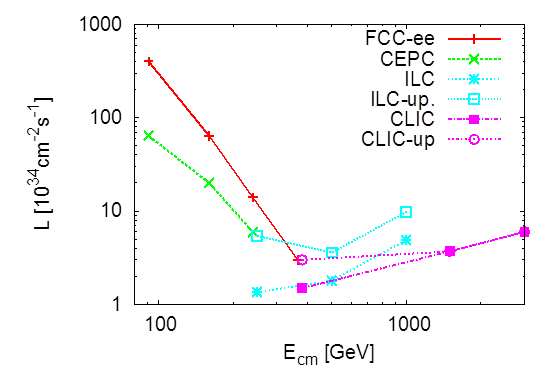
\includegraphics[width=0.9\textwidth]{\main/Accelerator/img/collider-luminosities.png}
\caption{Luminosity versus c.m.~energy for $e^+e^-$ Higgs Factories.
Two IPs are assumed for the circular colliders FCC-ee and CEPC.}
\label{luminosities}
\end{figure}


In order to achieve the luminosity, all colliders rely on very small beam sizes at collision (FCC-ee 30--70 nm, ILC 3--8 nm, CLIC 1--3 nm), well beyond those achieved at existing facilities  This requires very small beam emittances and ambitious focusing. Nanobeams are addressed via design and specifications, benchmarked simulations, low-emittance ring progress and studies, extensive prototyping and method developments (for alignment, stabilization, instrumentation and feedback systems, and algorithms), and in system and facility tests: FACET, light-sources, FEL linacs, ATF2).

In FCC-ee and CEPC the required emittance is achieved in the collider ring itself. FCC-ee and CEPC are based on a combination of concepts that have been proven and used in previous and present colliders. Some theoretical and experimental studies have been performed of critical effects, such as beam lifetime, beam-beam, impedances and electron cloud. Also, effects that have not been present in previous colliders have been studied, in particular the impact of beamstrahlung on the beam lifetime and instabilities. During the technical design phase, more complete studies, such as simulations of strong beam-beam effects with lattice imperfections, 
will be required to confirm this.

In ILC and CLIC the beam is produced in an injector and then cooled to small emittance in damping rings. The emittance targets for the damping rings have been achieved (and exceeded) with electron beams at modern light sources. A combination of technologies such as high-accuracy alignment, active magnet stabilization and beam-based alignment is designed to ensure that the emittance remains within budget during the beam transport to the collision point. Prototype tests at SLAC and KEK confirm the performance of the required beam-based alignment and tuning techniques, beam orbit and collision feedback systems, and beam focusing systems. 

In LCs 80\% polarisation of the electron beam is planned based on demonstrated performance in the SLC. ILC considers two alternative positron sources: a novel design based on undulators aimed at producing $\sim$30\% positron polarization, and a conventional design for unpolarised positrons. In CCs no polarisation of the colliding bunches is foreseen. 

Figure\ref{fig:schedules} shows possible schedules for the different facilities, including the option LHeC \cite{lhecid}. The LHeC proposal considers collisions of 7 TeV protons circulating in the LHC with 60 GeV electrons from a multi-turn high-current energy recovery linac (ERL). A corresponding ERL test facility (PERLE) \cite{perleid} is planned at LAL/Orsay. A similar $ep$ collider, based on the FCC-hh, is part of the FCC design (FCC-eh). In parallel, R\&D is presently proceeding for an electron-ion collider in the US \cite{eicid}. 
A possible variant or upgrade of FCC-ee using an ERL scheme has recently been proposed \cite{bnl-erl}, promising higher luminosity at higher energy, 
but this is still at a very preliminary stage. 


 \begin{figure}[ht]
 \centering
 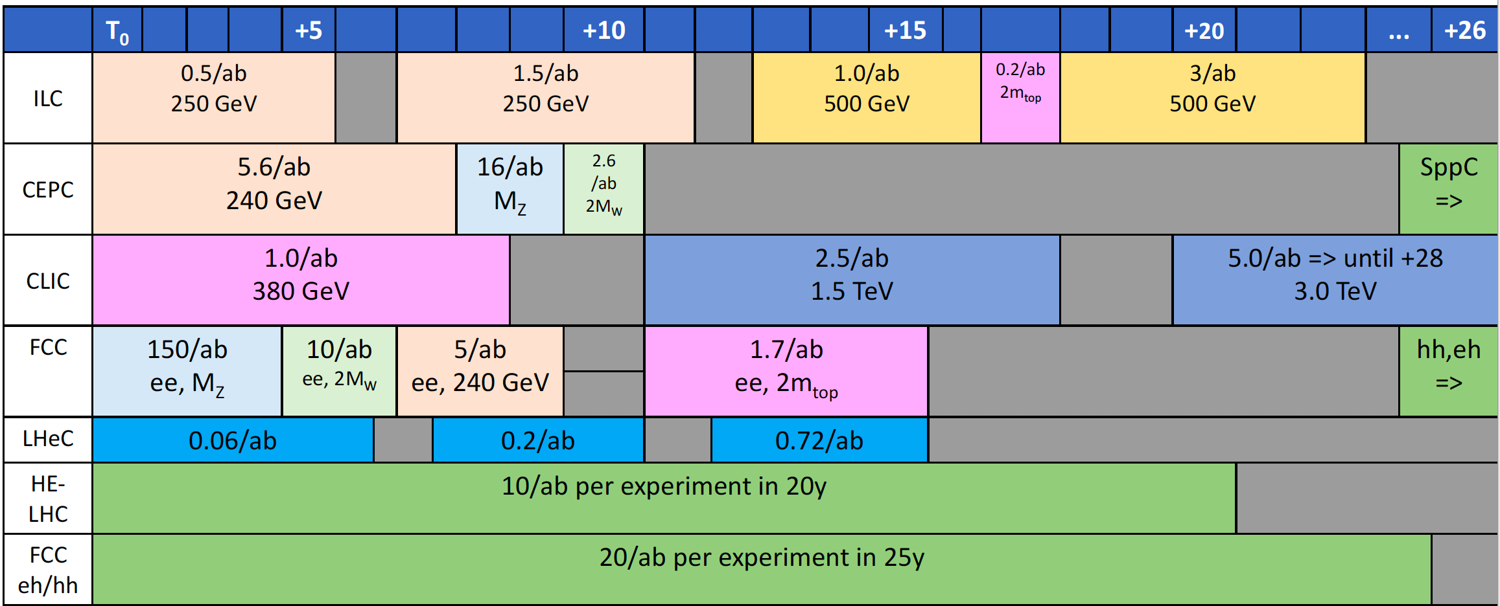
\includegraphics[width=0.75\textwidth]{\main/Accelerator/img/schedules.png}
 \caption{Timelines of various collider projects, in years and starting at time $T_0$ \protect\cite{heinemann}. --- {\bf Beate will change the starting year of SPPC}}
\label{fig:schedules}
\end{figure}

The main challenges for both LCs and CCs are the RF (energy) and nanobeam (luminosity) performances, but here there are strong synergies with modern synchrotron and FEL light-source requirements. The importance of these connections among electron accelerators with their broader science applications, and impact of collaborations among key European (and overseas) partner national institutes cannot be overstated.

\paragraph*{Linear colliders}

The LC initial stage provides a cost-effective and fast access to $e^+e^-$ collisions by 2035 for Higgs, top-quark and both SM and BSM studies. Such a machine leaves the door open for study of higher energy machines (LC extensions, and circular proton/muon colliders), for possible implementation on the 2040--50 timescale. The interplay between an evolving LC facility and a circular hadron, or possibly muon, collider---optimized in terms of technology, cost, size and first and foremost physics capability---would provide the global particle physics community with powerful tools for the foreseeable future. This approach also establishes a number of key accelerator R\&D goals for the next 1--2 decades. The main design parameters of the two LC options are given in Table \ref{tab:ilc-clic}  and Figure \ref{fig:int-lumi-ee} shows the corresponding foreseen integrated luminosities.


\begin{landscape}
\begin{table}[htbp]
\caption{Parameters for ILC and CLIC stages}
\label{tab:ilc-clic}
\begin{center}
\begin{tabular}{l|ccc|ccc}
\hline\hline
 &  \multicolumn{3}{c|}{ILC} &
 \multicolumn{3}{c}{CLIC} \\
 \hline
  & initial & L upgrade  &  500 GeV &  stage 1 & stage 2 & stage 3 \\
 \hline
 c.m.~energy [GeV] & 250 & 250 & 500 & 380 &
 1500 & 3000 \\
 rep.~rate [Hz] & 5 & 5/10 & 5 & 50 & 50 & 50 \\
 no.~bunches / pulse & 1312 & 2625 & 1312/2625 & 
352 & 312 & 312 \\
 bunch population [$10^{9}$] & 20 & 20 & 20 & 5.2 
 &  3.7 & 3.7
 \\
av.~beam current $I_b$ [$\mu$A] & 21  & 21/42 & 21/42 
& 15 & 9  & 9  \\ 
horizontal IP beta function $\beta_{x}^{\ast}$[mm]
& 13 & 13 &11 & 8 & 8 & 6 \\
vertical IP beta function $\beta_{y}^{\ast}$ [mm]
& 0.41 & 0.41 & 0.48 &  0.1 & 0.1 & 0.07 \\
horizontal geometric emittance at IP $\varepsilon_{x}$ [pm]
& 20 & 20 & 20 & 3 & 0.4 & 0.2  \\
vertical geometric emittance at IP $\varepsilon_{y}$ [fm]
& 140  & 140 &  70 & 80 & 14 &  7\\
horizontal rms IP beam size [nm] & 516 & 516 & 474 & 
149 & $\sim$60 &  $\sim$40\\
vertical rms IP beam size [nm] & 7.7 & 7.7 & 5.9 & 
2,9 & $\sim$1.5 &  $\sim$1\\
total luminosity $L$ $10^{34}$~cm$^{-2}$s$^{-1}$ &
1.35 & 2.7/5.4 & 1.8/3.6 & & & \\
luminosity in top 1\% $L_{0.01}/L$ & 
73\% & 73\% & 58.3\% &  60\% & 38\% & 34\% \\
Electrical site power [MW] &  115 & 135/185 &
163 & 170 & 290 & 580 \\
Site length [km]  &  20.5 & 20.5/31 & 31 & 
11.4 & 29.0 & 50.1  \\
Integrated luminosity [fb$^{-1}$/year]	
& 100 & 300 & 600 & 180 & 444 & 708\\
\hline\hline
\end{tabular}
\end{center}
\end{table}
\end{landscape}



\begin{figure}[ht]
\centering
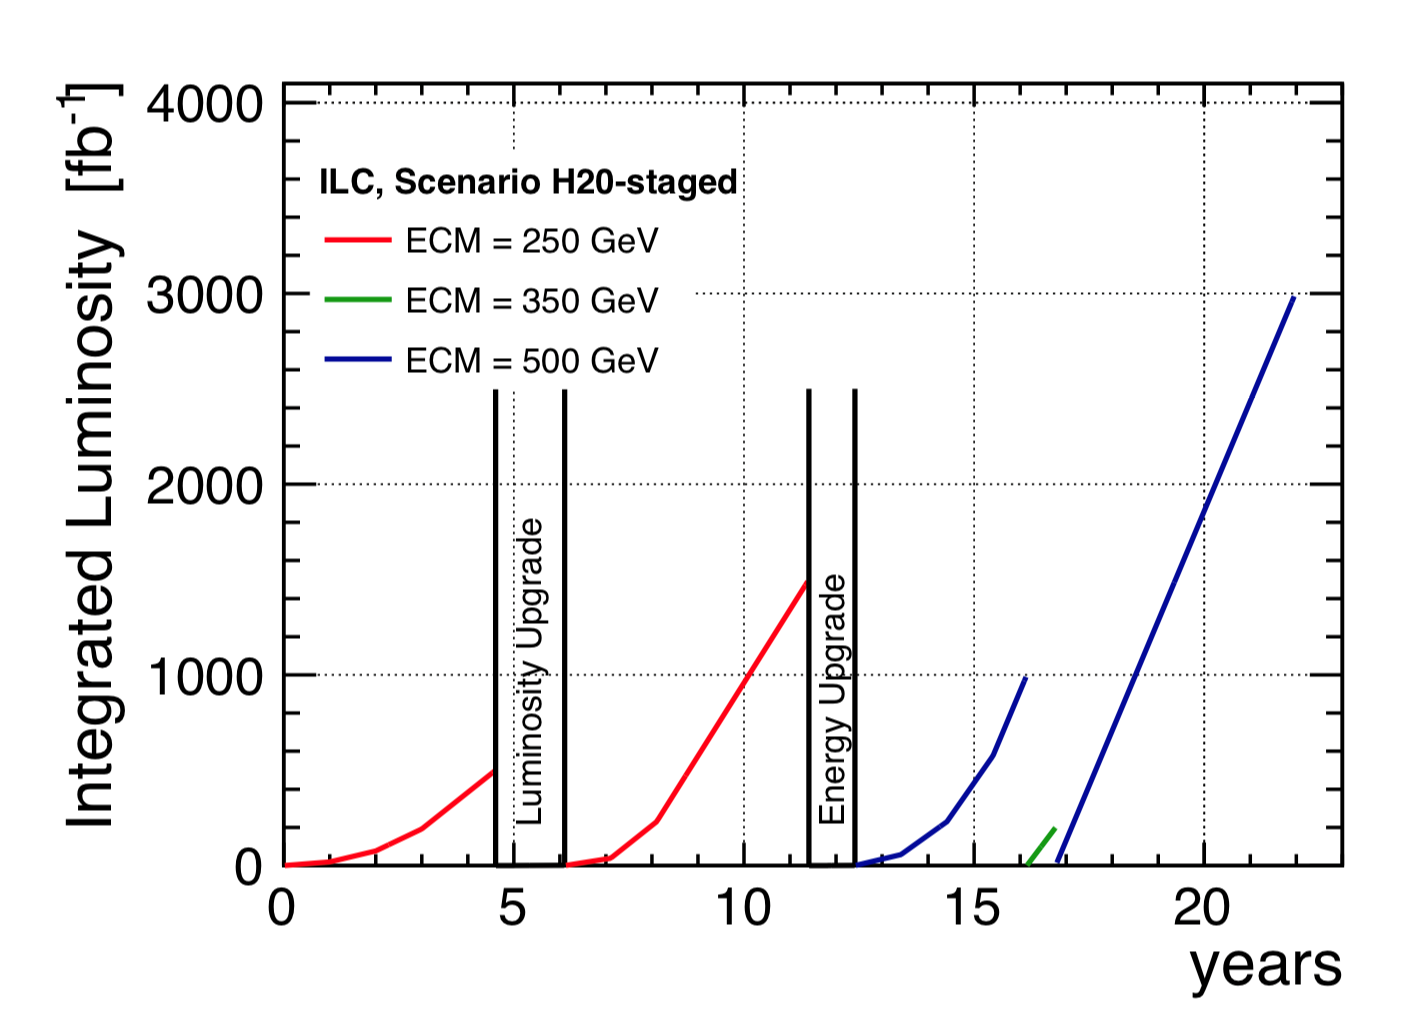
\includegraphics[width=0.32\textwidth]{\main/Accelerator/img/ilc-int-year.png}
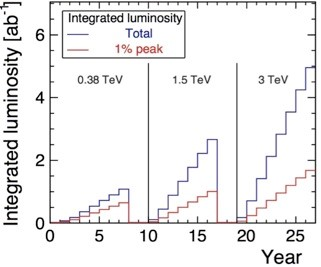
\includegraphics[width=0.32\textwidth]{\main/Accelerator/img/clic-int-year.jpg}
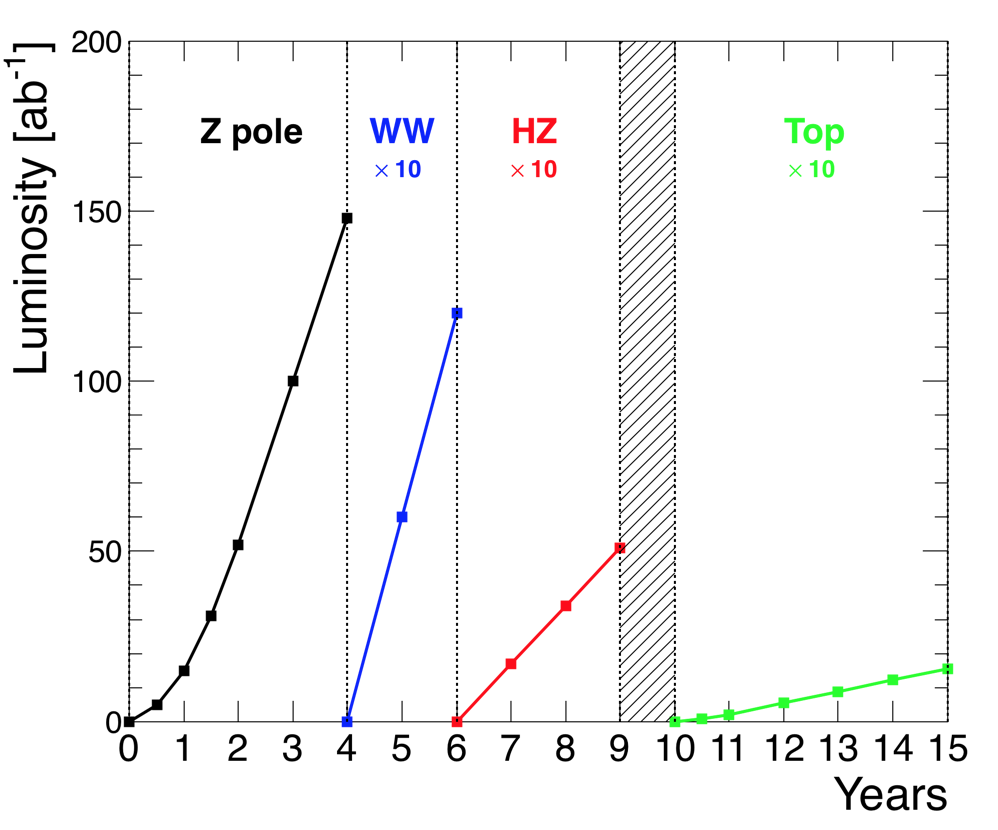
\includegraphics[width=0.32\textwidth]{\main/Accelerator/img/int-fccee-year.png}
\caption{Foreseen integrated luminosities of ILC, CLIC and FCC-ee versus year.}
\label{fig:int-lumi-ee}
\end{figure}



The proposals for CLIC [ID146] and ILC [ID77] are mature and complete, covering design of the accelerators, including their upgrades to higher energies, technical developments for critical systems, performance verification studies and detailed project implementation plans. There are strong communities supporting both project studies and proposals, as well as comprehensive detector and physics studies. Key features of these proposals include: the initial stages have costs and power budgets on a similar scale as LHC, making them well suited for rapid implementation; they can be readily expanded both in terms of energy---with existing, improved or novel RF technologies---and luminosity; polarized beams are foreseen; they can also be operated at lower energies (for example at the Z-pole, albeit with much lower luminosity than the CCs) and gamma-gamma collisions are possible. The physics performance is covered elsewhere in this document. Following discussions at the Granada symposium CLIC and ILC have submitted updated information about their Z-pole performances and luminosity upgrade options \cite{Latina:2687090,ilc-zpole-2019}.



{\bf CLIC} is proposed to be implemented as a CERN-hosted international project (following the LHC and HiLumi-LHC models) in three energy stages, 380, 1500 and 3000 GeV in the centre of mass (Table 2) with design luminosities between 1.5 and 5.9$\times 10^{34}$~cm$^{-2}$s$^{-1}$. A recent study for the initial stage \cite{Latina:2687090} shows that increasing the bunch train frequency by a factor 2 could double the luminosity, with only modest increases in the power 
($\sim 50$ MW) and cost ($\sim 5$\%). The CLIC timeline includes a preparation phase 2020--2025, followed by a 7-year construction and commissioning period, in order to be ready for data-taking before 2035. The CLIC$_{380}$ cost is estimated at 5.9 BCHF, with upgrade costs of +5 and +7 BCHF for the two further stages. The AC power of the initial (final) stage is estimated at about 170 MW (580 MW). Only the CLIC$_{380}$ power estimate has so far been optimized.

{\bf Dual-beam acceleration} has been demonstrated at CTF3 [ref]. Gradients of up to 200 MV/m have been achieved with {\bf normal-conducting RF} Cu technology; numerous CLIC X-band cavities have been operated at the design gradient of 100 MV/m and X-band RF technology is now well established and industrially available.  There is also underpinning experience with C-band for large-scale systems, e.g.~SwissFEL, including the production processes for the accelerator structures with demonstrated design performance. 

{\bf ILC } is proposed to be built for initial operation at 250 GeV, with a direct upgrade path to 500 GeV, and a possible further upgrade to 1000 GeV (Table 2). The luminosities foreseen are 1.35--4.9$\times 10^{34}$~cm$^{-2}$s$^{-1}$;  increasing the bunch train frequency by a factor 2 for the initial stage could double the luminosity while increasing the power by only 20--30 MW and the cost by $\sim$8\% \cite{michizono}. The timeline includes a preparation phase of 4 years, followed by a 9--10 year construction and commissioning period, in order to be ready before 2035. The ILC$_{250}$ cost is estimated to be 4.8--5.3 BILCU (ILCU = 2012 USD or 1.12 times 2019 USD), while ILC$_{500}$ would be around 8 BILCU. The AC power is estimated at about 130 MW (300 MW) for 250 GeV (1000 GeV). The ILC is foreseen to be constructed as a Japan-hosted international project. Relevant European capabilities and the scope of possible participation have been presented [ID66]. 

Over the last decades excellent progress has been has made with {\bf superconducting RF} technology, driven primarily by and for TESLA, ILC and then successfully implemented at EU-XFEL [REF] at DESY. The EU-XFEL represents a large-scale deployment of SC cavities  made by industry; many cavities exceed the design gradient of $\sim$23 MV/m, and some reach over 40 MV/m, which exceeds the ILC design gradient of 35 MV/m. EU-XFEL, together with the on-going construction of LCLS-II at SLAC provide a development and testing ground for key elements (e.g.~magnets, instrumentation, controls, and vacuum systems), with parameters close to those needed for ILC. Further technology optimization is ongoing, linked to evolving SCRF R\&D for improved cavity gradient and Q values. 
 

\paragraph*{Circular Colliders}

Circular $e^+e^-$ collider proposals build upon 50 years of experience. The designs of FCC-ee and CEPC exploit the historical knowledge from LEP (high energy), KEKB (high current, high luminosity, strong e+ source), PEP-II (high current), DA$\phi$NE (crab waist), and SuperKEKB (extremely low $\beta_{y}^{\ast}$, large Piwinski angle), and SLC (damping rings, powerful $e^+$  source). CCs can accommodate several interaction points (IPs); two IPs are assumed in the FCC-ee and CEPC baselines and an alternative design with 4 IPs is under development for FCC-ee.

Parameters for the stages of FCC-ee and CEPC are summarized in Table 3\ref{tab:fcc-cepc}. 
FCC-ee foresees starting on the $Z$ pole and then upgrading the RF systems in stages with optimized machine configuration for $Z$, $WW$, $ZH$, and $t\overline{t}$ working points. CEPC plans initially to install the full RF system for Higgs production, and later to operate on the $Z$ pole and then at the WW threshold. CCs have the potential for an extremely high production rate of $Z$ bosons (Tera $Z$ factory) and exquisite precision energy calibration at the $Z$ pole (100 keV) and at the $WW$ threshold using resonant depolarization.
The total FCC-ee construction cost (for $Z$, $W$ and $H$ working points) is estimated to be 10.5 BCHF [ID132]; operation at the $t\bar{t}$ working point will require later installation of additional RF cavities and associated cryogenic cooling infrastructure for an additional cost of 1.1 BCHF. The precision of the overall cost estimate is at the 30\% level. The annual energy consumption is similar to that of HL-LHC, and varies between 1 and 2 TWh. The total cost of CEPC was reported as 5 billion USD \cite{wang,cepc}. It should be noted that in each case both civil engineering and technical infrastructures can largely be reused for a subsequent hadron collider (FCC-hh or SPPC).

Each of the CC main concepts and parameters has been demonstrated in a previous collider (see earlier). Therefore, the CC designs are mature and R\&D is focussed on engineering optimization towards easing operability, machine efficiency, and maintainability aiming at efficient and cost-effective exploitation. R\&D includes highly efficient SC RF systems, high power RF couplers and high-efficiency RF power production all of which profit from past investments in a range of RF user communities. For FCC-ee a hybrid-technology solution has been found using Nb-sputtered Cu cavities for lower energies (as those first developed for LEP) operated at 4.5 K, combined with bulk Nb cavities for higher energies (profiting from ILC R\&D), operated at 1.8 K.  Other CC R\&D includes novel ultra-thin NEG coatings for the vacuum system, radiation shielding of accelerator components (coils, bellows, flanges), a feasible design of the machine-detector interface (MDI) and an energy efficient, cost effective magnet system for the collider arcs.

A performance upgrade of FCC-ee (luminosity increase by about 80\%) could be implemented via doubling the number of IPs from 2 to 4, without any effect on the circulating beam current and minimal impact on power consumption 
\cite{shatilov-2019,oide-2019,zimmermann-pol}. 
CEPC [ID51] considers a luminosity upgrade through increasing the SR power per beam from 30 to 50 MW (i.e.\ to the FCC-ee design value). A potential upgrade option with much higher gains both in luminosity (up to a factor 100) and energy (beyond 500 GeV) through conversion to an ERL-based collider was proposed recently \cite{bnl-erl}; its feasibility and cost must be studied in greater detail. 


\begin{landscape}
\begin{table}[htbp]
\caption{Parameters for FCC-ee and CEPC stages}
\label{tab:fcc-cepc}
\begin{center}
\begin{tabular}{l|cccc|ccc}
\hline\hline
 & \multicolumn{4}{c|}{FCC-ee} &
 \multicolumn{3}{c}{CEPC} \\
 \hline
 & stage 1 & stage 2 & stage 3 & stage 4 & stage 1 & stage 2 & stage 3 \\
 \hline
 c.m.~energy [GeV] & 91 & 160 & 240 & 350 / 365 &
 240 & 91 & 160 \\
 beam current [mA] & 1390 & 147 & 29 & 6.4 / 5.4
 &  17.4 & 461	& 87.9 \\ 
 Horizontal~emittance [nm]& 0.27 & 0.84 & 0.63& 1.34 /  1.46 & 1.21 & 0.18 & 0.54 \\
Vertical IP beta function [mm]
& 0.8 & 1.0 & 1.0 & 1.6 & 1.5& 1.0& 1.5\\
RF voltage [GV]	& 0.1 & 0.75 & 2.0 & 4.0+5.4 / 6.9 &  2.17 & 0.10& 0.47 \\
RF frequency [MHz]& 400	& 400 & 400 &  400 + 800 & 	\multicolumn{3}{c}{650} \\ 
RF cavities	& 1-cell Nb/Cu
& 	4-cell Nb/Cu
	& 4-cell Nb/Cu 	& 4-cell Nb/Cu (4.5 K) + 	& 
\multicolumn{3}{c}{2-cell bulk Nb}\\
& 
(4.5 K)& 	
(4.5 K)	&  (4.5 K)	& 5-cell bulk Nb (1.9 K)	& 
\multicolumn{3}{c}{(1.9 K)}\\
Peak luminosity (for two IPs) & 460 & 56& 17& 3.6 / 3.1
& 6 & 64 & 20 \\
\; \;  [$10^{34}$~ cm$^{-2}$s$^{-1}$] & & & & & & & \\
SR power / beam [MW] & 50 & 50 & 50 & 50 & 30 & 30 & 30 \\
Electrical power [MW] &  259 & 277 &
282 &	$\sim$350 & 270 & 149 & 223 \\
Run time [years] &  4 & 1--2 & 3 &1 / 4 &	
7 & 2 & 1 \\
Total integrated luminosity [ab$^{-1}$]	
& 150 & 10 & 5& 0.2 / 1.5 & 5.6 & 16 & 2.6\\
\hline\hline
\end{tabular}
\end{center}
\end{table}
\end{landscape}


\paragraph*{Complementary circular colliders}

{\bf SuperKEKB}~[ref], the KEKB upgrade, is presently under commissioning. Its design is based on the nanobeam collision scheme in a large Piwinski angle regime. It aims at $L = 80 \times 10^{34}$~cm$^{-2}$s$^{-1}$, increasing 
beam currents up to 3.6 and 2.6 A ($e^-$ and $e^+$ respectively), decreasing $\beta_{x,y}^{\ast}$  
to the level of 30 and 0.3 mm (H and V respectively) and decreasing the emittance to about 4 nm. 
SuperKEKB will test, and go beyond, many of the parameters of FCC-ee and CEPC, as the vertical design beta function, the Touschek positron beam lifetime (3 minutes, to be compared with an expected beam lifetime of 20--60 min in FCC-ee due to radiative Bhabha scattering), the higher beam currents and the higher production rate of positrons.

The design of the {\bf Super Tau-Charm Factory} (SCT) [ref] at BINP, Novosibirsk, is a collider with luminosity of 
$10^{35}$~cm$^{-2}$s$^{-1}$ at centre of mass energy between 2 GeV and 6 GeV with the possibility to exploit longitudinally polarized electrons at the interaction point (IP), for production of charmonium and tau-lepton domain. It is based, as the FCC-ee on the Crab Waist collision scheme. 



\section{Path towards highest energies}
For the foreseeable future, proton-proton collisions appear to offer the greatest collision-energy reach, up to roughly 100 TeV. Table \ref{tab:ppcoll} summarizes the major parameters and technical challenges for possible future proton colliders. Their realization depends both on high-field superconducting magnets, for which major R\&D is required, and on the provision of a large circular tunnel. Such a tunnel could also be used to house a lower-energy proton collider based on e.g.~6 T single-layer Nb-Ti magnets at 1.9 K, or a much lower-energy $e^+e^-$ collider (see above). A high-energy linear $e^+e^-$ collider, i.e.~ILC$_{1000}$ or CLIC$_{3000}$, described above, can also push the physics reach in lepton collisions towards and beyond that of the LHC (see Chapters~\ref{chap:ew} and \ref{chap:bsm}). Electron-hadron colliders, i.e.~LHeC or FCC-eh, could incorporate one ring of the proton collider and a new electron linac based on e.g.\ LC linac technology or an ERL. Muon colliders need substantial R\&D (see Section \ref{sec:muon}); if realizable, they have the potential to reach collision energies up to a few tens of TeV. Plasma-based wakefield acceleration also offers long-term possibilities for reaching high energies (see Section \ref{sec:plasma}).


\begin{table}[htbp]
\caption{Parameters of proposed future high-energy hadron colliders HE-LHC, FCC-hh and SPPC.
\label{tab:ppcoll}
}
\begin{center}
\begin{tabular}{lccc}
\hline\hline
&  HE-LHC & FCC-hh & SPPC  \\
\hline
Beam Energy [TeV]&
        13.5 & {50} &
        {37.5}\\
Circumference [km] &
        26.7 & {97.75} &\\
Interaction regions  &
	 2(+2) & 2+2 &	
        {2}   \\ \hline
Integrated lumi.\ per main experiment [ab$^{-1}$/yr]  &
0.5 & 
        {0.2--1.0} &
        {0.4}  
         \\ 
Peak luminosity [10$^{34}$/cm$^{2}$/s] & 
16 & 
        {5--30}&  
        {10} 
 \\
Time between collisions [ns]&
25 & 25 & 25 \\
Energy spread [rms, $10^{-3}$]&
0.1 &
        {0.1} &
        {0.2} \\
Bunch length [rms, mm]&
80 & 
        {80}&
        {75.5} \\
RMS IP beam size [$\mu$m]&
6.6 &
        {6.8 (initial.)}& 
        {6.8 (initial)}
 \\
Injection energy [TeV]&
1.3 & 
	{3.3}&
	{2.1}  \\ 
Transverse geometric emittance [rms, nm]&
0.17 (init.) & 
        {0.04 (init.)}&
        {0.06 (init.)}
        \\ 
$\beta^*$ at IP [cm] &
45 & 
        {110--30 }&        
        {75} \\ \hline
Beam-beam parameter/IP [$10^{-3}]$ &
12 & 
         {5--15}&
         {7.5}\\
RF frequency [MHz]&
400 & 
	{400}&
	{400/200} \\
Particles per bunch [$10^{10}]$ &
22 & 
        {10}&
        {15}0 \\
Bunches per beam  &
2808 & 
        {10600}&
        {10080} \\
Average beam current [mA]  &
1120 & 
        {500}&
        {730}\\
Length of standard arc cell [m]  &
137 & 
        {213}&
        {148}\\ \hline
Peak magnetic field [T]  &
16 & 
        {16}&
        {12}\\
SR power loss/beam  [MW] &
0.1 & 
	{2.4}&
	{1.1} \\ \hline\hline
	\end{tabular}
	\end{center}
\end{table}

The most critical requirement for a high-energy collider is energy reach and the proposed ILC$_{1000}$ and CLIC$_{3000}$, or HE-LHC, FCC-hh and SppC, offer the highest energies in electron and proton collisions, respectively. Relevant criteria for feasibility of implementation are cost, AC power, and the required R\&D effort. The construction costs and AC power estimates are all within a factor 2--3 of each another. Nominally the lowest cost is for HE-LHC, followed by ILC$_{1000}$, CLIC$_{3000}$ and FCC-hh. The AC site power consumption is the lowest for HE-LHC, followed by ILC$_{1000}$, FCC-hh and CLIC$_{3000}$.  In terms of the required duration/scale of the R\&D effort to reach a TDR level of readiness, CLIC$_{3000}$ and a version of HE-LHC based on HL-LHC 12 T magnet technology are ahead of other proposals, and require roughly 10 years of R\&D/design optimization;  roughly twice that time will be required for the baseline 16 T HE-LHC and FCC-hh.

The hardest challenge for the proton colliders is the development of a representative magnet with maximum 16 T field. There are fundamental challenges in obtaining the required current density in superconductors and in dealing with the ultimate magnetic pressures and mechanical stresses in the superconductor and associated components. One can estimate the timescale needed to innovate new approaches/technology and overcome these limits through continual R\&D efforts [see also Fig.~\ref{fig:hctl}], as follows:

\begin{enumerate}

\item 
    Nb$_3$Sn, 14 T to 16 T (25-28 TeV @ LHC, 90-100 TeV @ FCC-hh):  10--15 years for short-model R\&D, and the following 10 to 15 years for prototype/pre-series with industry, resulting  result in 20–30 years before a construction  start.

\item Nb$_3$Sn, 12 T to 14 T (21-25 TeV @ LHC, 75-90 TeV @ FCC-hh):  7--10 years for short-model R\&D, and an additional 7--10 years for prototype/pre-series with industry, resulting in 15–-20 years before a construction start. The technical feasibility to reach 14 T has been demonstrated recently via the short-model FRESCA-2 project in Europe and the MDP programme in the US, yielding an accelerator-type cos-theta short dipole model with 4-layer coil geometry (as for the FCC 16 T design).

\item Nb$_3$Sn, 9 T to 12 T (16-21 TeV @ LHC, 55-75 TeV @ FCC-hh): based on experience with the HL-LHC 11 T dipole and IR quadrupole magnets, a few years for short-model R\&D, and an additonal few years for prototype/pre-series with industry, resulting in construction feasibility in 5--10 years.

\item  NbTi, 6 T to 8 T (35-50 TeV @ FCC-hh): NbTi 8 T dipole magnets are very similar to the current LHC main dipole with two-layer coils, and 6 T magnets may be the cheapest option by using a single-layer cos-theta coil winding. After reasonable prototyping work, including optimization based on the existing proven technology, both options could be available for construction within 5-7 years. 
\end{enumerate}

Because of its much higher current density capability, High Temperature Superconductor (HTS) technology will inevitably be required to reach fields beyond 16 T. A critical limitation of HTS today is its much higher cost, even compared with Nb$_3$Sn, however Nb$_3$Sn is already available as an industrial product, and HTS technology will presumably mature in the future.

{\bf Something of the beam power + helium consumption?}

 \begin{figure}[ht]
 \centering
 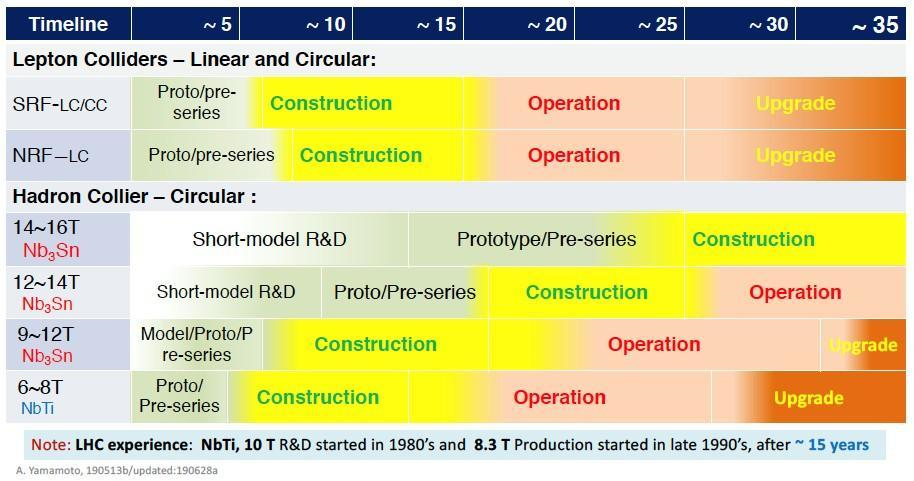
\includegraphics[width=0.75\textwidth]{\main/Accelerator/img/hc-timeline.png}
\caption{ A relative timeline expected for realizing future lepton and hadron colliders (from A.~Yamamoto, presented at the Open Symposium in Granada, and updated based on the discussion followed).}
\label{fig:hctl}
\end{figure}

\section{Muon Colliders}
\label{sec:muon}
A muon collider \cite{muonid} has the potential to reach attractive luminosities in very high-energy lepton collisions. It would be a powerful discovery machine, since, in contrast to a proton collider, the full collision energy is available in the centre of mass. The higher muon mass reduces synchrotron radiation emission and allows for the acceleration and collision of the beams in a circular facility, permitting a much lower integrated RF voltage per turn and efficient use of the beams for luminosity production. A muon collider promises a linear increase of the luminosity per unit beam power with increasing collision energy, in contrast to a LC where it is independent of the collision energy. A circular collider also allows the possibility of multiple collision points, thereby mitigating the large AC power consumption at very high energies. In addition, the luminosity spectrum could be substantially better than for an $e^+e^-$ LC due to the strongly reduced beamstrahlung and initial state radiation. 

Two main muon collider concepts have been proposed: in one the muons are generated using protons (MAP) \cite{Delahaye:2013jla,accel:muon3-sr1} 
in the other using positrons (LEMMA) \cite{Antonelli:2015nla}\cite{accel:lemma2019}. The proton-driven scheme was the object of a well-supported study, mainly in the US, but the effort was suspended about five years ago. The recently proposed positron-driven scheme is being studied with a limited effort mainly at INFN. Since no organised collaboration exists for muon colliders, a review group has been charged to assess their perspectives and status. This review is based on the material made available by the MAP and LEMMA studies and on some additional calculations. 
Figure \ref{fig9} shows the dependence of the luminosity per unit beam power for the proton-based muon collider in comparison with $e^+e^-$ colliders. 

The proton-driven scheme is based on classical muon production via pion decay. The study has addressed the global collider parameters and several key technical issues, such as fast-ramping magnets and RF cavities in a high magnetic field. Although it has not reached the level of a CDR, it is sufficiently complete to give confidence in the collider parameters. In the positron-driven scheme, 45 GeV positrons impinging on electrons at rest in a target produce muon pairs close to the reaction threshold, hence with a very low emittance. Two issues in the original LEMMA study have recently been identified that potentially reduce the luminosity by orders of magnitude. The LEMMA team is performing a redesign of the collider concept to address these issues but it is too early to assess the results.

The decays of the accelerated muons drive critical issues:
\begin{itemize}
\item	
At the collision points, the decay electrons induce a large background of electrons and photons. A first simulation study with realistic conditions indicates that this background can be mitigated by suitable shielding, detector design, and analysis, such that it would not damage the physics capability.
\item	
The neutrinos from muon decays along the ring produce showers in the Earth. This leads to some radiation at the location where the plane of the collider ring intercepts the Earth's surface. At very high energies beyond 6 TeV, this could ultimately limit the achievable luminosity for the proton-based scheme. The positron-driven scheme would be particularly attractive in this respect since its smaller emittance requires much smaller beam current and thus reduces the neutrino dose, enhancing further the possible energy reach.
\end{itemize}


Although a muon collider offers the potential to push the energy frontier beyond the capabilities of any other conventional approach currently considered, the concept is not mature enough to be considered for construction today. A strong R\&D programme would be needed to develop it as a possible candidate for a high-energy physics project. This would be synergistic with R\&D on topics such as high-field superconducting magnets, fast-ramping magnets, efficient superconducting RF, and normal-conducting high-field RF; other topics , such as crystal collimation, might also be important.

A possible direct source of low-emittance muon or intense positron beams could be the ``Gamma Factory'', where partially stripped heavy ions stored in the LHC (or in the FCC-hh) are collided with a laser pulse to generate intense bursts of X-rays.  Initial studies in the LHC have demonstrated an excellent lifetime of the partially stripped ion beam \cite{id6}.

A conceptual R\&D programme is illustrated in Figure \ref{fig:muonrd}. In the first stage, the baseline collider concept would be developed in parallel with the specification of a major R\&D project that could address the key technical issues, possibly including some physics goals using high-intensity muon or neutrino beams. This phase would require relatively modest resources. A consortium of interested institutes, including CERN, is starting to form. Due to the challenging design issues the project provides an excellent opportunity to nurture new ideas and  skills for the future. Depending on the results of this stage one could launch the second stage (6 years) in which one or more test facilities could be built and operated. The collider design could be further optimised and a CDR developed, including costing, and used as the basis for a decision on whether to proceed to the next (4 year) TDR stage, at which point a decision on construction could be taken. On this basis it is possible to imagine operation of a muon collider more than roughly 25 years from now. The formation of a global collaboration will be essential to carry out the work coherently and efficiently. 

 \begin{figure}[ht]
 \centering
 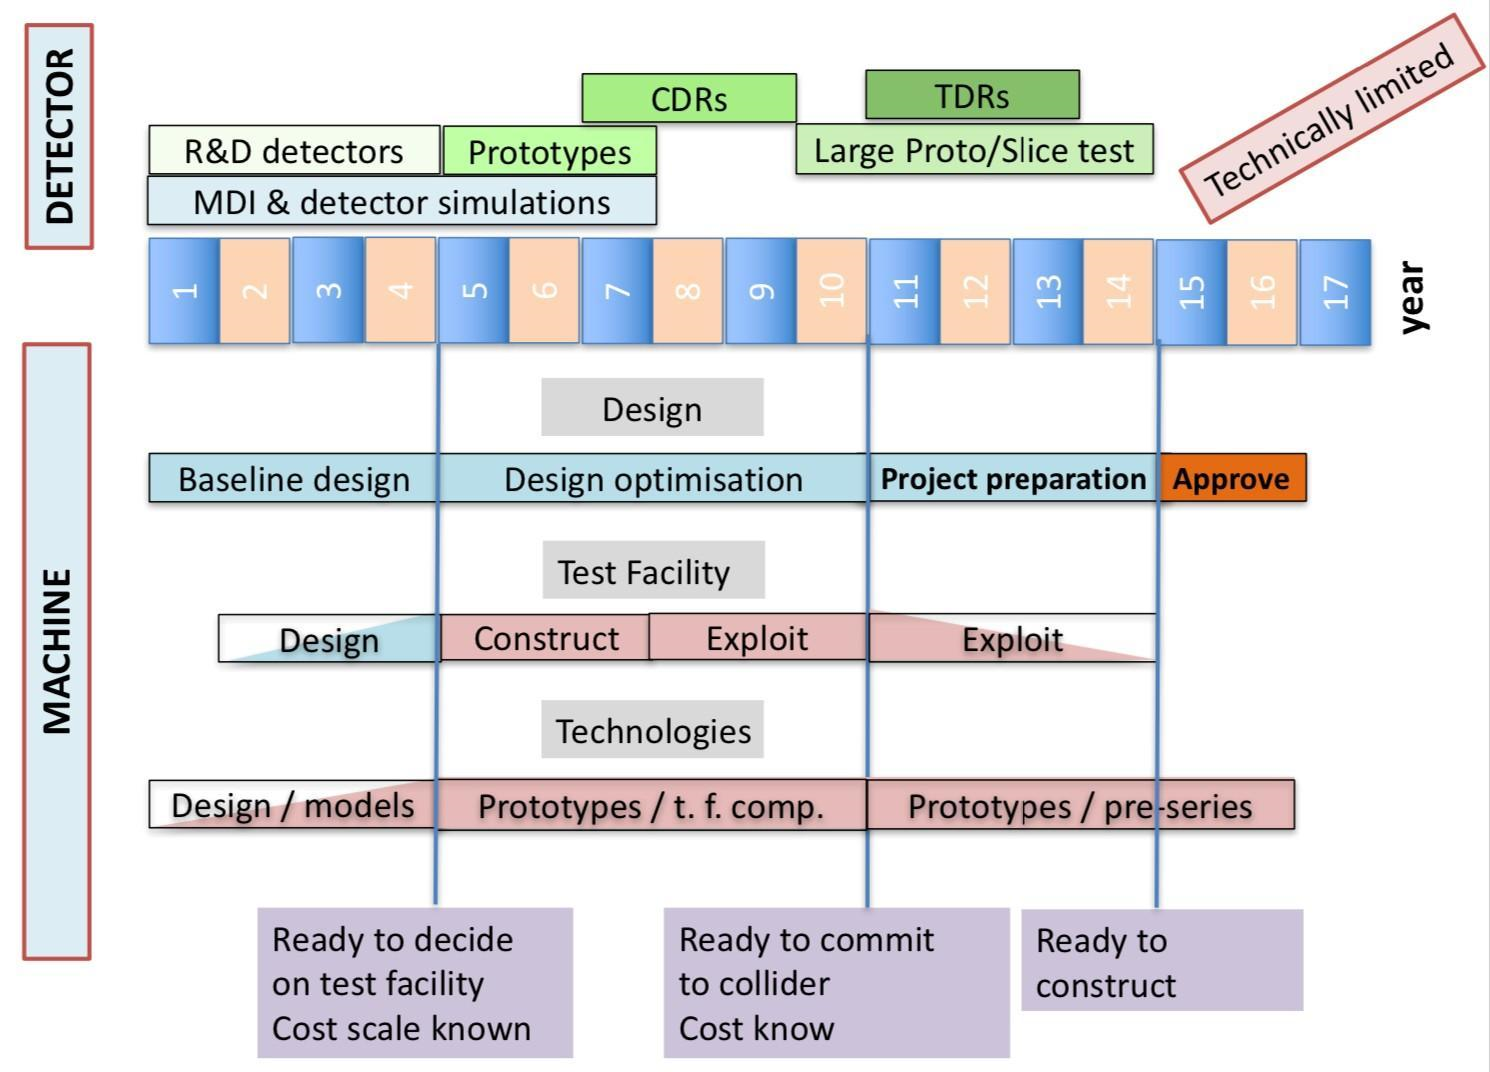
\includegraphics[width=0.75\textwidth]{\main/Accelerator/img/muon-rd-tl.png}
 \caption{Potential technically limited timeline for a muon collider.}
\label{fig:muonrd}
\end{figure}

\section{Plasma acceleration}
\label{sec:plasma}
Accelerating gradient is one of the key elements in determining the energy reach and the size of any accelerator. RF cavities accelerating gradients range from few MeV/m up to the value demonstrated in CLIC test facilities of over 100 MeV/m. Plasma-based particle accelerators, where accelerating fields are created by the collective motion of plasma electrons driven by lasers or particle beams, have shown capability of reaching an order of magnitude higher gradients. A myriad of applications of such technology would benefit from the compactness of the devices, HEP of course being  one the interested fields.

\paragraph*{Present status of the field}

In the past decade significant progress has been made on both laser- and particle-beam-driven plasma accelerators.

\noindent{\it Laser-driven:} With the emergence of PW class lasers, electrons up to 8 GeV have been generated from 20 cm long plasma structures \cite{wim2} and staging of two independently powered modules has been demonstrated at the 100 MeV energy level \cite{wim3}. Methods for reduction of electron-beam energy spread from initially few percent to a few tenths of a percent have been developed \cite{wim4,wim5}, and emittances at the 0.2 micron have been measured. Strong plasma-based focusing elements have been developed and optimized which provide symmetric high gradients at the few kT/m level \cite{wim6,wim7,wim8} that are emittance preserving \cite{wim9}. Sophisticated diagnostics that are able to probe plasma profiles, accelerating and focusing fields as well as the properties of the emerging femtosecond electron beams, with high temporal resolution \cite{wim10} are being developed. Continuous operation of laser plasma accelerators operating at the 1 Hz repetition rate with energy stability at the few percent level has been demonstrated over extended times (>24 hrs), and an understanding of the origin of fluctuations has been obtained, permitting a path to feedback stabilization when increasing the repetition rate to kHz and beyond \cite{wim11}.

\noindent{\it Electron-driven:} Electron-driven plasma acceleration has shown energy doubling of a fraction of a beam from 42 GeV to 85 GeV in an 85 cm-long plasma column \cite{wim12}. Single-stage acceleration of a full electron beam by 9 GeV has been achieved \cite{wim13}, and sub-percent energy spread and 30\% energy transfer efficiency from the drive to the accelerated beam has been demonstrated \cite{wim14}. The acceleration of positron bunches was realized in a quasi-linear wakefield \cite{wim15} and energy gain of 5 GeV with an energy spread at the per cent level was reached \cite{wim16}.

\noindent{\it Proton-driven:} The possibility of using relativistic proton beams as a driver was demonstrated at the CERN AWAKE experiment \cite{wim17}: although the proton beams have much longer bunch length, it was shown \cite{wim18,wim19} that they self-modulate in plasma to micro-bunches which can resonantly drive wakefields. The acceleration of electrons to multi-GeV energies in a 10m-long plasma was demonstrated \cite{wim17}.

For colliders, the hosing mechanism, equivalent to beam break-up, has been analyzed in depth and mitigation strategies have been developed to ensure suppression of this important instability \cite{wim20,wim21}. Tolerance studies on alignment of beams and structures are being conducted to understand the operational parameter regimes and challenges that need to be overcome \cite{wim22}. Advances have been made in speeding up the computational tools, with the aim of reducing the computation time from multiple days to minutes. This has been achieved via the development of advanced computational methods, reduced models that capture the essential physics, and through the emergence of higher-speed computers.

The latest generation of beam-driven plasma accelerators is utilizing superconducting accelerator technology and deploying feedback systems and advanced controls for the synthesis of finely tuneable and stable drive beams. They are now entering the era of precision measurements with sub-percent beam energy stability and fine beam-loading control for energy-spread minimization.  These activities are accompanied by the exploration of repetition rate limits for plasma-wakefield processes facilitated by accelerator technology for multi-MHz and high- average power operation.

\paragraph*{Challenges}

The next ten years of advanced accelerator development will focus on addressing challenges identified by the community:
\begin{enumerate}
\item	
Demonstration of reliable 24/7 operation of GeV-class plasma-based accelerators producing high quality electron beams with low energy spread (<\,0.5\%), low emittance (<\,1 micron) and high charge per bunch (>\,30 pC) in femtosecond bunches.
\item	
Higher energy staging of electron acceleration with independent drive beams, equal energy, and charge-preserving beam capture; optimization of external injection methods.
\item	
Understanding mechanisms for emittance growth and developing methods for achieving emittances that are compatible with colliders.
\item Energy efficiency studies and optimization.
\item Demonstration of high average power operation for both beam- and laser-driven plasma accelerators;
\item Completion of a single electron acceleration stage at higher energy (10 GeV).
\item Demonstration and understanding of methods to accelerate a positron bunch with good quality.
\item Demonstration of scalable electron acceleration to 10s of GeV, with emittance control, via proton-driven plasma wakefield acceleration, leading to first high-energy physics applications.
\item Construction of dedicated advanced and novel accelerator facilities in order to deliver reliably high quality, multi-GeV electron beams from a small number of stages.
\item Energize the advanced accelerator community, including the HEP community, towards an advanced collider.
\item Continual development of a comprehensive and realistic operational parameter set for a multi-TeV collider.
\item For the laser-driven scheme, the development of a MW-level (average power) laser system, which is 4-5 orders of magnitude higher than what is available today.
\item Further studies of beamstrahlung effects for c.m. energies up to 10 TeV. 
\end{enumerate} 

\paragraph*{Advanced Accelerator Concept roadmap}

 The primary long-term goal of a multi-TeV collider sets a timescale for the Advanced Accelerator Concepts (AAC) roadmap for completion of a TDR in the 2035-2040 interval \cite{wim1}.
 
\noindent{\it Near-term goals:} completion of a TDR for a potential early application in the 2025-2030 interval. During the innovation and discovery phase, the focus will be on generating and preserving high quality electron bunches, methods for producing and efficient capture of positron beams, long distance acceleration and scalability of plasmas for particle beam driven wakefields, studies on energy efficiency, suppression of instabilities, and many other topics. Early applications include compact and possibly transportable Thomson scattering based gamma-ray sources, compact FELs, medical radiation delivering devices, and radiation-based inspection accelerators. In addition, laser plasma accelerators could be considered as injectors for next generation diffraction limited light sources.

\noindent{\it Mid-term goal:} the AWAKE technology could provide particle physics applications: AWAKE Phase 2 could be used for fixed target experiments for dark photon searches as well as to deliver future electron-proton or electron-ion collisions with low luminosity.

\noindent{\it Long-term goal:} design of a high-energy electron/positron/gamma linear collider based on laser- and/or beam-driven plasma wakefield acceleration.


\section{Accelerators Beyond Colliders}

\paragraph*{Accelerator-based Neutrino Beams}

High energy and high beam power accelerators are extensively used for neutrino physics research. The cost of leading facilities is second only to colliders. (for reference, total project cost (TPC) of J-PARC \cite{id76} is about 1.7 B\$, the cost estimate of the proposed ESS$\nu$SB \cite{id98} is 1.3 BEuro.)

At present, the leading operational facilities are the Fermilab Main Injector complex that delivers over 0.75 MW of 120 GeV protons on the neutrino target, and the J-PARC facility in Japan which recently approached 0.5 MW of the 30 GeV proton beam power.

Both facilities have multi-MW upgrade plans: Fermilab---through construction of a new 0.8 GeV PIP-II linac (to achieve over 1.2 MW by 2026) and then PIP-III (either an 8-12 GeV RCS or an SRF linac to achieve >2.4 MW in mid-2030's); 
J-PARC---through new faster magnet power supplies to reduce the cycle from 2.48s to 1.32s and RF upgrade to e.g. 1.3 MW by 2028. Far future plans of the J-PARC team include the construction of a new 8-GeV Booster in addition to their existing 3 GeV RCS to attain 3.2 MW out of the Main Ring (MR), and even, still later, a new 9 MW 9-GeV proton driver consisting of three SRF linacs (1.2 GeV, 3.3 GeV and 6.2 GeV) in the straight sections of the KEKB tunnel which will be available after the conclusion of the Super KEK B-factory operation. It is of note that the Proton Driver for the Energy Frontier muon colliders, like the proposed 14 TeV c.m. energy muon collider in the LHC tunnel, will need to operate at 2 to 4 MW average power level. 

Two issues are currently not resolved so that one cannot yet claim feasibility of these upgrades or any other multi-MW facilities: a) target; b) beam losses.

The long list of issues associated with high power targets is further compounded by the fact that the required beam impacts are very short---1 to 10 microseconds. As a result, the countermeasures against radiation damage (DPAs) and thermal shock-waves at the existing neutrino targets and horns work only up to $\sim$0.8 MW of beam power. MW and multi-MW targets are under active development and prototyping. Ongoing R\&D programs include studies of material properties, new forms (foams, fibers), new target designs (e.g., rotating or liquid targets). This R\&D activity has common elements with target R\&D for other HEP frontier projects (dark sector searches, linear collider, positron-based muon collider/LEMMA) and requires coordinated support.

The other most stringent limits on the beam power are set by the need to lower the fractional beam losses while increasing the beam power. The tolerable uncontrolled beam loss in accelerator enclosures is typically about 1 W/m, so the fractional beam loss must be kept under $\Delta N/N\sim C({\rm ircumference})\times 1 (W/m) /P({\rm ower})$. 
Such demands are in gross contradiction with the commonly observed increase of the $\Delta N/N$ with intensity, caused, e.g.\ by space-charge effects. 

These issues are very serious, are being addressed \cite{Shiltsev19}, and require long-term support of dedicated accelerators, machine studies, theory and modeling efforts.

There are four new proposals submitted to the EPPSU which show significant scientific promise and should be further studied---Protvino/ORKA, ENUBET, $\nu$STORM and ESS$\nu$SB. The first two call for moderate expansion of existing facilities and operation at sub-MW power levels. $\nu$STORM (cost est.\ 160~MEuros if built at CERN) will produce beams of electron and muon antineutrinos from the decay of muons confined within a 580 m racetrack shape storage ring. It requires only 156kW of 100 GeV protons and the major challenges of the proposal is the necessity of large diameter (0.5 m) magnets to accept most of the secondary muons and a sophisticated focusing lattice which should assure survival of about 60\% of muons with 10\% rms momentum spread over 100 turns. $\nu$STORM represents a very promising approach with great potential to boost R\&D toward energy frontier muon colliders.

ESS$\nu$SB is a technically very challenging proposal with a total cost of some 1.3 B Euros. It calls for an increase of the ESS beam power from the world record design value of 5 MW to 10 MW by increasing the accelerator duty cycle from 4\% to 8\%; the additional 5 MW are used to generate a uniquely intense neutrino Super Beam for the measurement of leptonic CP violation. The use of ESS \cite{id164} for search for baryon number violation \cite{id156} is also proposed. Beside the upgrade of the SRF linac repetition rate from 14 Hz to 28 Hz, ESS should switch from operation with protons to operation with H$^-$ particles. An accumulator ring with 400 m circumference will need to be built to compress to the beam pulse to one microsecond. Due to very short beam pulse, the required 5MW neutrino target station will be much more challenging than the 5 MW ESS neutron spallation target. One should also expect---and address---very strong space charge effects both in the linac and in the accumulator ring. High power H$^-$ stripping would also be a challenge.


\paragraph*{BSM Searches with Accelerators}

Many of the BSM experiments could be based on existing accelerator facilities, like SPS, LHC, PSI, FNAL, etc. A few others would require new dedicated accelerators, such as an EDM ring. As per the conclusions of the Physics Beyond Colliders (PBC)/BSM reports [arXiv:1902.00260, ID20, ID42, ID60], and illustrated in Figure \ref{fig:bsm},  the BSM proposals broadly break down along the lines of:

\noindent{\bf \it  Sub-eV Axion/ALP searches} [ID112]: Here the main thrusts are well-established:
\begin{itemize}
\item	Helioscopes (BabyIAXO/IAXO);
\item	Haloscopes (Resonant cavities e.g. ADMX, MADMAX);
\item Light-shining-through-walls (JURA, STAX);
\item Oscillating EDMs in protons or deuterons in an electrostatic ring (an idea rather than a proposal at the moment, cf.\ CPEDM measurement proposal below) [ID18].
\end{itemize}

\noindent{\bf \it MeV-GeV mass range:}
\begin{itemize}
\item	Direct detection WIMP searches;
\item	Proton beam dump: new proposals (SHiP \cite{id12,id129}), re-purposed existing experiments (NA62, MiniBooNE, SeaQuest);
\item	Electron beam dump: NA64 \cite{id9}, LDMX \cite{id36}, BDX, RedTop 
\cite{id28} \ldots  
\item	Long lived particles at the LHC (FASER, MATHUSLA, CODEX-b, MilliQan).
\end{itemize}

\noindent{\bf \it $\gg$TeV mass range:}
\begin{itemize}
\item Ultra-rare or forbidden decays (KLEVER \cite{id153}, TauFV \cite{id102}, Mu3e, MEG...);
\item Search for a permanent EDM in protons/deuterons (CPEDM) or in strange/charmed baryons (LHC-FT).
\end{itemize}

Proposed BSM/PBC experiments at CERN and elsewhere, e.g.~COMET at J-PARC \cite{id38}, are compiled in Tables \ref{tab:BSMsummary} and \ref{tab:BSMOthers}, 
 respectively. The competitiveness of all CERN PBC options are explored in depth in the BSM paper \cite{Alemany:2019vsk}, which includes wide-ranging evaluation covering 11 benchmark cases. Also see the PBC summary report for the European Strategy Update \cite{id20}.

 \begin{figure}[t]
 \centering
 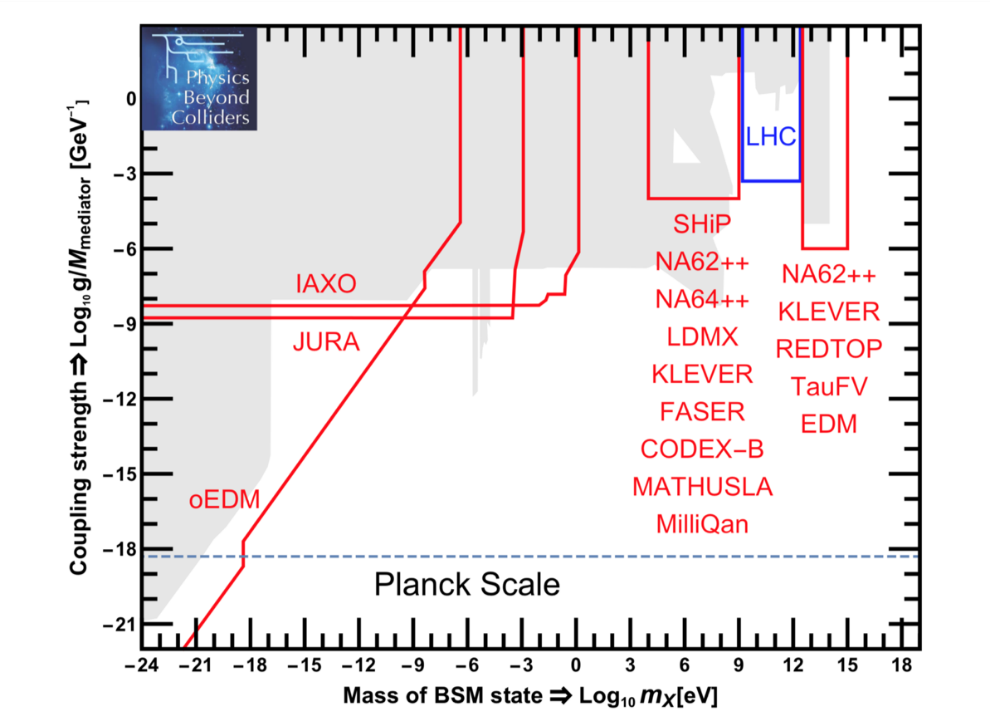
\includegraphics[width=0.75\textwidth]{\main/Accelerator/img/bsm.png}
\caption{BSM parameter space---PBC options shown, general breakdown maps onto worldwide options.}
\label{fig:bsm}
\end{figure}

Concerning the compatibility of experiments with beam from the CERN SPS, an SPS operation model has been fully developed for North Area. In general, the SPS could only support one major user in addition to standard North Area operation. The operation of BDF/SHiP/TauFV \cite{id12,id129,id102} is compatible with standard NA operation (and LHC, AWAKE, HiRadMat, MD). The operation of BDF/SHiP/TauFV is compatible with standard NA/KLEVER operation with some compromise. Similar conclusions hold for NA/KLEVER with eSPS/LDMX. The eSPS/LDMX is not compatible with full BDF/SHiP operation. And either $\nu$STORM or ENUBET would not be compatible with BDF---a temporal separation will be necessary.

As for the possible time line of SPS-based experiments, the conventional SPS beam program is foreseen for execution over LHC Run 3/Run 4. KLEVER and COMPASS$^{++}$ with RF separated beams both require significant investment and development. Data taking would be in Run 4 at the earliest.
If approved, BDF/SHiP would target construction starting circa 2025. Ideally, BDF would make use of the injectors' LS3 (2025) to perform key civil engineering work during the associated NA stop. Realistically the earliest SHiP could start taking data is mid-Run 4.
If approved, eSPS would ideally target construction in the next 5 years. eSPS could potentially execute its program before SHiP data taking, but this would require strong commitment by CERN within the next 2 years or so, followed by prompt technical design, approval, and execution.
$\nu$STORM and ENUBET, given their present limited implementation studies, and CERN's other commitments, cannot be envisaged to start construction until after 2030.


\begin{landscape}
\begin{table}[h]
\begin{center}
\caption{Projects considered in the PBC-BSM working group categorised in terms of their sensitivity to a set of benchmark models in
a given mass range. The characteristics of the required beam lines, whenever applicable, are also displayed. Copied from BSM report. }
\label{tab:BSMsummary}
\begin{tabular}{lllcc}
\hline
Proposal &    Main Physics Cases  & Beam Line  & Beam Type  & Beam Yield \\
\hline
\textbf{sub-eV mass range:}:  &  &  &  & \\
\hline
IAXO  & Axions/ALPs (photon coupling)  & –  & axions from sun &  – \\
JURA  & Axions/ALPs (photon coupling)  & laboratory  & eV photons  & –  \\
CPEDM  & $p$, $d$ EDMs  & EDM ring  & $p$, $d$  & –  \\
 &  Axions/ALPs (gluon coupling) &  &  $p$, $d$  & – \\
 
LHC-FT  & charmed hadrons EDMs  & LHCb IP  & 7 TeV p  &  – \\
\hline
\textbf{MeV-GeV mass range:}  &  &  &  & \\
\hline
SHiP  & ALPs, Dark Photons, Dark Scalars &  BDF, SPS  & 400 GeV $p$  & \num{2e20}/5 years \\
 & LDM, HNLs, lepto-phobic DM, .. &  &  & \\
 
NA62++  & ALPs, Dark Photons,  & K12, SPS  & 400 GeV $p$  & up to \num{3e18}/year \\
 & Dark Scalars, HNLs  &  &  &  \\
 
NA64++  & ALPs, Dark Photons,  & H4, SPS  & 100 GeV   $e^\text{-}$  & \num{5e12} eot/year \\
& Dark Scalars, LDM  &  &  & \\
& + L$_\mu$ -- L$_\tau$  & M2, SPS  & 160 GeV $\mu$  & \num{e12}-\num{e13} mot/year \\
& + CP, CPT, leptophobic DM  & H2--H8, T9  &  ~40 GeV $\pi$, $K$, $p$  &  \num{5e12}/year \\

LDMX  & Dark Photon, LDM, ALPs,...  & eSPS  &  8(SLAC)-16(eSPS) GeV $e^\text{-}$  & \num{e16}-\num{e18} eot/year \\

AWAKE++  & Dark Photon  & AWAKE beam  & 30-50 GeV $e^\text{-}$  & \num{e16} eot/year \\

RedTop  & Dark Photon, Dark scalar, ALPs  & CERN PS  & 1.8 or 3.5 GeV $p$ & \num{e17} pot \\

MATHUSLA200  & weak-scale LLPs, Dark Scalar,  & ATLAS or CMS IP  & 14 TeV $p$  &  3000 fb\textsuperscript{-1} \\
& Dark Photon, ALPs, HNLs  &  &  & \\

FASER  & Dark Photon, Dark Scalar, ALPs,  & ATLAS IP &  14 TeV $p$  & 3000 fb\textsuperscript{-1} \\
 & HNLs, B--L gauge bosons &  &  & \\

MilliQan  & milli charge &  CMS IP &  14 TeV $p$  & 300-3000 fb\textsuperscript{-1} \\

CODEX-b  & Dark Scalar, HNLs, ALPs,  & LHCb IP  & 14 TeV $p$  & 300 fb\textsuperscript{-1} \\
 & LDM, Higgs decays  &  &  & \\
\hline
\textbf{>> TeV mass range:}  &  &  &  & \\
\hline
KLEVER & $K_L \rightarrow \pi^0\nu\bar{\nu}$  & P42/K12  & 400 GeV $p$  & \num{5e19} pot/5 years \\
TauFV  & LFV $\tau$ decays  & BDF  & 400 GeV $p$  & O(2\%) of the BDF proton yield \\

CPEDM  & $p$, $d$ oEDMs &  EDM ring  & $p$, $d$ &  – \\
 & Axions/ALPs (gluon coupling)  & & $p$, $d$  & – \\

LHC-FT  & charmed hadrons MDMs, EDMs  & LHCb IP  & 7 TeV  $p$ & \\


\hline
\end{tabular}
\end{center}
\end{table}
\end{landscape}

\newpage

\begin{landscape}
\begin{table}[h]
\begin{center}
\caption{Selection of projects complementary to those considered by PBC-BSM working group. Note that the experiments are in different phases: proposals; construction; upgrades. (BD -- beam dump; SX -- slow extraction; DD -- direct detection) }
\label{tab:BSMOthers}
\begin{tabular}{lllcc}
\hline
Proposal &    Main Physics Cases  & Beam Line  & Beam Type  & Beam Yield \\
\hline

\textbf{sub-eV mass range:}:  &  &  &  & \\
\hline

%Axions etc 
MADMAX & Axions & Lab - dielectric/B field & cosmos & - \\
STAX & ALPs  & LSW sub-THz photons &  cosmos  & -\\
MAGIS100$\rightarrow$1K & Dark sector & Atom interferometer (FNAL) & cosmos &  - \\

\hline
\textbf{MeV-GeV mass range:}  &  &  &  & \\
\hline

% Direct WIMP searches
DARKSIDE-20k$\rightarrow$Argo  & WIMP DD LAr & LNGS & cosmos & 200 t.yr $\rightarrow$ 3000 t.yr\\
DARWIN & WIMP DD LXe & possibly LNGS & cosmos & 200 t.y \\
LUX-ZEPLIN (LZ) & WIMP DD LXe & SURF & cosmos & 15 t.y \\
XENONnT & WIMP DD LXe & LNGS  & cosmos &  20 t.y\\
CRESST-III Phase 2  & WIMP DD, A' CaWO$_4$ & LNGS & cosmos &  - \\
SuperCDMS & WIMP DD Ge & SNOLAB & cosmos & - \\
% beam dumps
SEAQUEST BD & LDM & FNAL MI & 120 GeV $p$ SX &   \num{1.44e18} pot/2 years \\ 
MiniBooNE-DM & LDM & FNAL Booster & 8 GeV/c $p$ & \num{1.9e20} pot \\
BDX & LDM, A' & JLAB  & 11 GeV $e$  & \num{e22} eot \\
DarkLight &	 A' & JLAB  & 100 MeV $e$ on $p$ & 5 mA \\
SENSEI & LDM   & CCDs (FNAL/SNOLAB)  & cosmos & - \\
MAGIX & A' & MESA  & 150 MeV $e$  & $\sim$\num{e35} cm\textsuperscript{-2}s\textsuperscript{-1} \\
MMAPS &  $e^\text{-}e^\text{+}\rightarrow \gamma A'$ & Cornell synchrotron & 5.3 GeV $e^\text{+}$ SX &  $L_{av} =$ \num{0.9e34} cm\textsuperscript{-2}s\textsuperscript{-1}    \\	
BELLE-II & ALPS, A' & SuperKEKB  & $e^\text{-}$$e^\text{+}$ $\sqrt{s}$ = 10.58 GeV  &   50 ab\textsuperscript{-1}\\

%APEX &  dark photons  & & & \\


\hline
\textbf{>> TeV mass range:}  &  &  &  & \\
\hline

Mu3e I/II & CLFV $\mu^+\rightarrow e^+e^+e^-$  & PSI HiMB &  $\mu$ & \num{2e9} stopped $\mu$/s \\

MEG II & CLFV $\mu^+\rightarrow e^+\gamma$  & PSI &  $\mu$ &  $O$(\num{e10} $\mu$/s) to exp. \\

KOTO(+)  & $K_L \rightarrow \pi^0\nu\bar{\nu}$ & J-PARC MR SX   & 30 GeV $p$ 50$\rightarrow$100 kW   &  $\sim$\num{e8} K/spill@50 kW   \\

Mu2e/Mu2e-II &  CLFV $\mu^-N\rightarrow e^-N$ & FNAL & x GeV  $p\rightarrow\mu$ & 7.7 kW pot(phase I) \num{6.7e17} $\mu$  \\

COMET I/II & CLFV $\mu^-N\rightarrow e^-N$ & J-PARC MR  & 8 GeV $p\rightarrow\mu$ & \num{1.5e16} - \num{1.8e18}  stopped $\mu$ \\

\hline
\textbf{Acc. driven $\nu$ experiments}  &  &  &  & \\
\hline
% accelerator driven neutrinos
DUNE & $\nu$ & FNAL MR (PIP-II) & 60-120 GeV $p$  & 1.1$\rightarrow$1.9$\times$\num{e21} pot/yr\\
T2HK & $\nu$ & J-PARC MR & 30 GeV $p$ & $\sim$\num{1e21} pot/yr \\



\hline
\end{tabular}
\end{center}
\end{table}
\end{landscape}



\section{Energy management}

All proposed HEP projects will consume large amounts of energy, O(TWh⁄y). On the other hand, an increasing fraction of sustainable energy sources like wind and photovoltaics in the future energy mix will result in strong variations of the supply of electrical energy. It is HEP community responsibility to develop sustainable models and optimized technologies in terms of energy consumption, aiming also at exporting improved technologies for other application in the society.

One way to mitigate the impact of HEP facilities is to actively manage their energy consumption. The aim should be to avoid high loads on the grid during low supply conditions, and instead using preferentially ``excess energy''. The possibilities of energy management using dynamic operation of facilities and energy storage systems should be studied in more detail.

It is necessary to invest R\&D efforts improving the energy efficiency of HEP facilities through critical technologies. In certain areas, such R\&D will have an immediate impact on research and other facilities operated today, and the savings in energy consumption may be used to co-finance the investments. Certain improved technologies may also serve the society directly. These relevant fields of R\&D include (but are not limited to) optimized magnet design, high efficiency RF power generation, improved cryogenics, lower loss or higher operating temperature SRF cavity technology, beam energy recovery, district heating using recovered heat, and energy storage.

Proposals for future lepton colliders include linear colliders using normal-conducting or superconducting technology (CLIC and ILC), a large diameter synchrotron (FCC-ee) and muon colliders (MAP-MC). Defining the energy efficiency as integrated luminosity per supplied primary energy, these proposals have different dependencies on the targeted centre-of-mass energy. Figure \ref{fig9} shows the trends for these proposals, based on the numbers from the proposals submitted to the European Strategy Update. The absolute numbers presented should however be taken with caution, since the level of confidence and the degree of refinement for those proposals differ substantially. The overall trend however is based on fundamental principles and gives some indication. It shows the steep decrease of efficiency for the synchrotron radiation dominated FCC, and almost flat energy dependency for the linear colliders.


 \begin{figure}[ht]
 \centering
 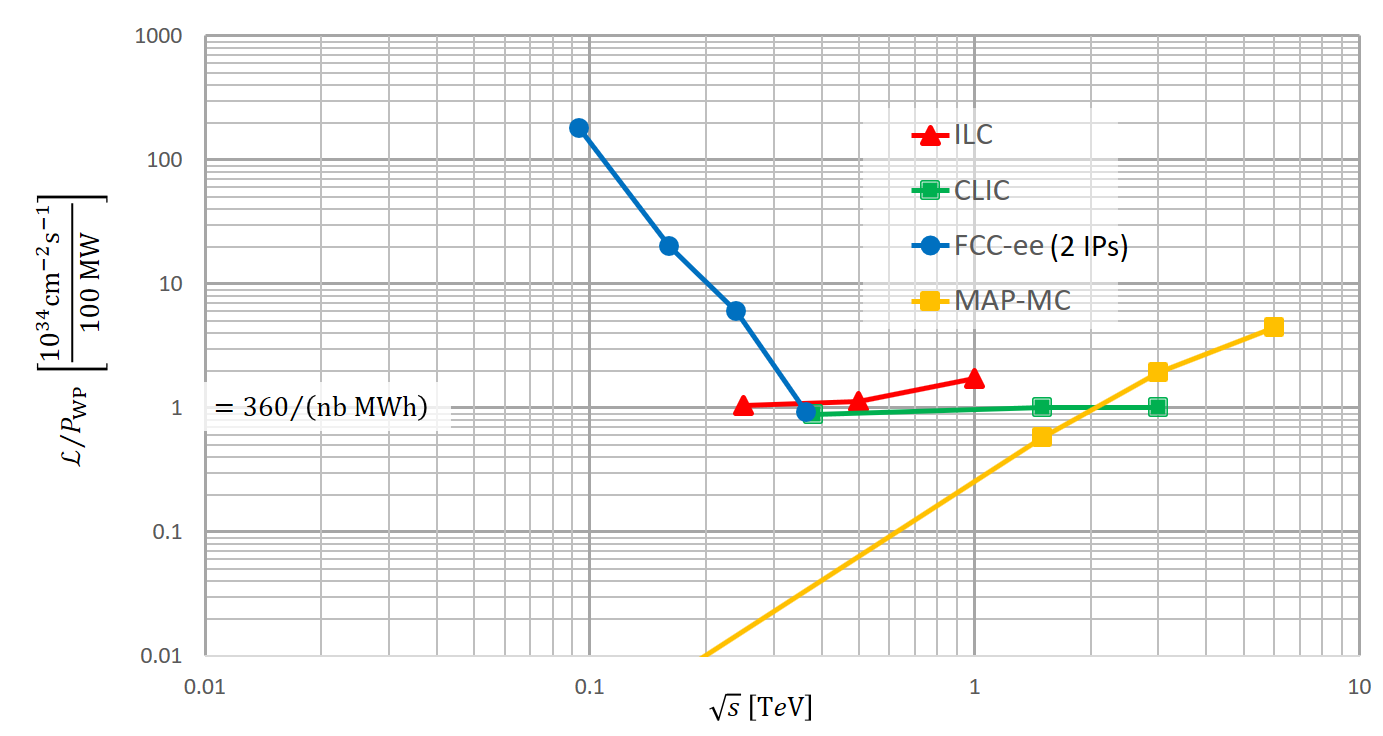
\includegraphics[width=0.75\textwidth]{\main/Accelerator/img/eneff.png}
\caption{One possible figure of merit for future colliders: luminosity per supplied primary energy (from E.~Jensen and M.~Seidel's presentation in Granada) \cite{jensen-granada}.}
\label{fig9}
\end{figure}


It should equally be taken into consideration that a highly optimized machine running   at its performance limit may have more significant downtime than a robust machine running very stably. In other words, energy efficiency of individual components is nothing without high system availability. The optimization should be on the overall performance, considering also the trade-offs between different subsystems and the effective Mean Time Between Failures (MBTF).


\section {Complementarities and synergies with other fields}
Accelerator technology development has always been driven by HEP needs. A diversity of other applications benefit from and synergistically contribute to the advances in the field. We mention here some of the most significant examples.

{\bf Fusion energy:} IFMIF and DONES accelerators, as complementary facilities to ITER project, are based on high power and high reliability proton linacs. They share with HEP project the challenges on high-intensity high-reliability proton and deuteron beam injectors; superconducting RF cavity technology in a high-power high-reliability context; high-intensity beam dynamics and beam halo understanding; high-power non-interceptive beam instrumentation; reliability modelling of particle accelerators. Their development has impact on industries building the systems, which reverts in capacitation and provider availaibility.

The {\bf HTS} \cite{HTSapps} technology has a wide variety of applications in medicine, science and power systems engineering on top of the High Field magnets, these last being also used in fusion power plants. As an example, HTS can apply in the field of electric power systems in cables, motors, generators, and transformers where superconductors replace resistive conductors, plus superconducting magnetic energy storage (SMES) and fault-current limiters (FCLs).

{\bf Medical applications} of accelerators in isotope production, radio and hadron-therapy \cite{PTCOG} are profiting of developments being carried out in HEP laboratories, and examples are the latest designs of SC gantries \cite{gatoroid}, \cite{Schippers}, or of medical detectors \cite{GEM}, \cite{DECTRIS}. 

{\bf Photonics and neutronics} share with HEP technologies and challenges. Common to all these fields are the high reliability needs and the data analytics evolution which exponentially grows in parallel to the high rep and detector capabilities. In photonics the examples are: the diffraction limited storage rings with very low emittance (nanobeam, stability, magnet and vacuum technology,...), the FELs (Linac technology, highly brilliant beam production and preservation, stability,...), the development of compact sources, where the CLIC technology has given birth to the  CompactFEL concept \cite{COMPACTLIGHT}. While in neutronics SNS, ESS or the China neutron source share with HEP all challenges of high power Linac and targets. 

And finally, as already mentioned above, {\bf plasma acceleration} promises developments for compact facilities with a wide variety of applications, in medicine, photonics, etc., compatible with university capacities and small and medium size laboratories.

An important aspect of this strategy update is to recognize the potential impact of the development of accelerator and associated technology on the progress in other branches of science, such as astroparticle physics, cosmology and nuclear physics. Moreover, joint developments with applied fields in academia and industry have brought about benefits to fundamental research and may become indispensable for the progress in our field.

% -- Add bibliography to table of contents
%\addcontentsline{toc}{chapter}{References}

% dummy reference to avoid that bibtex fails
% -- Add volume bibliography and part specific bibliographies
%\bibliographystyle{report}
%\bibliography{\bibfiles}

\end{document}




